
\subsection{Lista de materiales}

\begin{table}[h!]
\centering

\label{BOM}


\resizebox{0.99 \textwidth}{!}{

\begin{tabular}{|l|l|l|l|l|l|l|l|l|}
\hline
	Descripción & Nombre & Referencia & Potencia & Cantidad & Tipo & Tensión & Tensión de zener & Tolerancia \\ \hline
	TERMI-BLOK HEADER,ASSY90 2P - serie 282822 - 5.00mm & B1 & C-282822-2-C &  & 1 &  &  &  &  \\ \hline
	TERMI-BLOK HEADER,ASSY90 2P - serie 282822 - 5.00mm & B2 & C-282822-2-C &  & 1 &  &  &  &  \\ \hline
	TERMI-BLOK HEADER,ASSY90 2P - serie 282822 - 5.00mm & B3 & C-282822-2-C &  & 1 &  &  &  &  \\ \hline
	TERMI-BLOK HEADER,ASSY90 2P - serie 282822 - 5.00mm & B4 & C-282822-2-C &  & 1 &  &  &  &  \\ \hline
	TE Barrier Terminal Block, 2P & BO & 8PCV-02-006 &  & 1 &  & 600V &  &  \\ \hline
	Aluminum Electrolytic Capacitor 1000μF 16V 20\% 105º & CAF & Al. Elect. 1000u 16V 20\% 105º &  & 1 &  & 16V &  & 20\% \\ \hline
	Aluminum Electrolytic Capacitor 47μF 35V 20\% 105º & CAI & Al. Elect. 47u 35V 20\% 105º &  & 1 &  & 35V &  & 20\% \\ \hline
	Ceramic Capacitor 10nF 50V 10\% & CC1 & Cer. 10n 50V 10\% &  & 1 &  & 50V &  & 10\% \\ \hline
	Ceramic Capacitor 6.8nF 50V 10\% & CC2 & Cer. 6.8n 50V 10\% &  & 1 &  & 50V &  & 10\% \\ \hline
	Ceramic Capacitor 68pF 50V 10\% & CC3, CC4 & Cer. 68p 50V 10\% &  & 2 &  & 50V &  & 10\% \\ \hline
	Ceramic Capacitor 100pF 50V 10\% & CC5, CC6 & Cer. 100p 50V 10\% &  & 2 &  & 50V &  & 10\% \\ \hline
	Ceramic Capacitor 1.2pF 50V 10\% & CC7 & Cer. 1.2p 50V 10\% &  & 1 &  & 50V &  & 10\% \\ \hline
	Aluminum Electrolytic Capacitor 220μF 16V 20\% 85º & CCF32, CF31 & Al. Elect. 220u 16V 20\% 85º &  & 2 &  & 16V &  & 20\% \\ \hline
	Aluminum Electrolytic Capacitor 470μF 100V 20\% 105º & CF1, CF2, CF3, CF4, CF9, CF10 & Al. Elect. 470u 100V 20\% 105º &  & 6 &  & 100V &  & 20\% \\ \hline
	Polyester Capacitor 100nF 100V 10\% & CF5, CF6, CF7, CF8, CF11, CF12 & Poly. 100n 100V 10\% &  & 6 &  & 100V &  & 10\% \\ \hline
	Ceramic Capacitor 100nF 50V 10\% & CF33, CF34, CF37, CF38 & Cer. 100n 50V 10\% &  & 4 &  & 50V &  & 10\% \\ \hline
	Aluminum Electrolytic Capacitor 220μF 35V 20\% 105º & CF35, CF36 & Al. Elect. 220u 35V 20\% 105º &  & 2 &  & 35V &  & 20\% \\ \hline
	Tantalum Electrolytic Capacitor 1μF 25V 10\% & CF39, CF40 & Tant. Elect. 1u 25V 10\% &  & 2 &  & 25V &  & 10\% \\ \hline
	45 V, 16 A SWITCHMODE(TM) Schottky Power Rectifier, 2-Pin TO-220, Pb-Free, Tube & D1, D2 & MBR1645 &  & 2 &  &  &  &  \\ \hline
	FAST SWITCHING DIODE & D3, D4 & 1N4148 & 400mW & 2 &  &  &  &  \\ \hline
	FAST SWITCHING DIODE & D5, D6, D31, D32, D33, D34 & 1N4148 & 400mW & 6 &  &  &  &  \\ \hline
	SURFACE MOUNT FAST SWITCHING DIODE & D35, D36, D37, D38 & 1N4148W & 400mW & 4 &  &  &  &  \\ \hline
	Zener Diode, 2.7V, 500mW & DZ1, DZ2 & 1N4371A & 500mW & 2 &  &  & 2.7V &  \\ \hline
	Zener Diode, 22V, 500mW & DZ3, DZ4 & 1N969B & 500mW & 2 &  &  & 22V &  \\ \hline
	5V fixed regulator - 100mA & IC1 & LM78L05 &  & 1 &  &  &  &  \\ \hline
	-5V fixed regulator - 100mA & IC2 & LM79L05 &  & 1 &  &  &  &  \\ \hline
	Conn Phono Jack F 3 POS Solder RA Thru-Hole 3 Terminal 1 Port & JI & PJRAN1X1U01X &  & 1 &  &  &  &  \\ \hline
	Jumper Wire & JU1, JU2, JU3, JU4 & Jumper\_3pin &  & 4 &  &  &  &  \\ \hline
	Jumper Wire & JU5 & Jumper &  & 1 &  &  &  &  \\ \hline
	Typical LED (GREEN) & LED1 & LED (GREEN) &  & 1 &  &  &  &  \\ \hline
	Typical LED (YELLOW) & LED2 & LED (YELLOW) &  & 1 &  &  &  &  \\ \hline
	Transistor GP BJT NPN 230V 15A 3-Pin\_3+Tab\_ TO-264 Tube & Q1, Q3, Q5 & 2SC5200 & 150W & 3 &  &  &  &  \\ \hline
	Transistor GP BJT PNP 230V 15A 3-Pin\_3+Tab\_ TO-264 Tube & Q2, Q4, Q6 & 2SA1943 & 150W & 3 &  &  &  &  \\ \hline
	Plastic Medium-Power NPN Silicon Transistor, 300 VOLTS, 0.5 AMPERE, 20 WATTS & Q7, Q9, Q15, Q16, Q19 & MJE340G & 20W & 5 &  &  &  &  \\ \hline
	Plastic Medium-Power PNP Silicon Transistor, 300 VOLTS, 0.5 AMPERE, 20 WATTS & Q8, Q10, Q20 & MJE350G & 20W & 3 &  &  &  &  \\ \hline
	High Voltage NPN Bipolar Transistor & Q11, Q18 & MPSA42 & 20W & 2 &  &  &  &  \\ \hline
	High Voltage PNP Bipolar Transistor & Q12, Q17 & MPSA92 & 20W & 2 &  &  &  &  \\ \hline
	High Voltage NPN Bipolar Transistor & Q31, Q35, Q37 & MMBTA42 & 20W & 3 &  &  &  &  \\ \hline
	High Voltage PNP Bipolar Transistor & Q32, Q36, Q38 & MMBTA92 & 20W & 3 &  &  &  &  \\ \hline
	Quad NPN and PNP General-Purpose Amplifier & QI & MMPQ6700 & 180mW & 1 &  &  &  &  \\ \hline
	Resistor 0.1$\Omega$ 2W 5\% & R1, R2, R5, R6 & Resistor 0.1 2W 5\% & 2W & 4 & (TH) Carbon film &  &  & 5\% \\ \hline
	Cemented resistor 0.15$\Omega$ 5\% 5W & R3, R4 & Cemented resistor 0.15 5W 5\% & 5W & 2 & (TH) Wired cemented &  &  & 5\% \\ \hline
	Resistor 68$\Omega$ 1/4W 1\% & R7, R8 & Resistor 68 1/4W 1\% & 1/4W & 2 & (TH) Metal film &  &  & 1\% \\ \hline
	Resistor 100$\Omega$ 1/4W 1\% & R9, R10, R11, R12, R17, R18 & Resistor 100 1/4W 1\% & 1/4W & 6 & (TH) Metal film &  &  & 1\% \\ \hline
	Resistor 22K$\Omega$ 1/4W 1\% & R13, R14 & Resistor 22K 1/4W 1\% & 1/4W & 2 & (TH) Metal film &  &  & 1\% \\ \hline
	Resistor 30$\Omega$ 1/4W 1\% & R15, R16 & Resistor 30 1/4W 1\% & 1/4W & 2 & (TH) Metal film &  &  & 1\% \\ \hline
	Resistor 360$\Omega$ 1/4W 1\% & R19, R20 & Resistor 360 1/4W 1\% & 1/4W & 2 & (TH) Metal film &  &  & 1\% \\ \hline
	Resistor 510$\Omega$ 1/4W 1\% & R21, R22 & Resistor 510 1/4W 1\% & 1/4W & 2 & (TH) Metal film &  &  & 1\% \\ \hline
	Resistor 16K$\Omega$ 1/4W 1\% & R31, R32 & Resistor 16K 1/4W 1\% & 1/4W & 2 & (TH) Metal film &  &  & 1\% \\ \hline
	RES 150R SM0805 YAGEO RC\_L & R33, R34 & RC0805FR-07150RL &  & 2 &  &  &  &  \\ \hline
	Resistor 15K$\Omega$ 1/4W 1\% & R35, R36 & Resistor 15K 1/4W 1\% & 1/4W & 2 & (TH) Metal film &  &  & 1\% \\ \hline
	RES 1K2 SM0603 YAGEO RC\_L & R37, R38 & RC0603FR-071K2L &  & 2 &  &  &  &  \\ \hline
	Resistor 15$\Omega$ 1/4W 1\% & RF1, RF2 & Resistor 15 1/4W 1\% & 1/4W & 2 & (TH) Metal film &  &  & 1\% \\ \hline
	Resistor 36K$\Omega$ 1/4W 1\% & RFB1, RIOF & Resistor 36K 1/4W 1\% & 1/4W & 2 & (TH) Metal film &  &  & 1\% \\ \hline
	Resistor 1.3k$\Omega$ 1/4W 1\% & RFB2 & Resistor 1.3k 1/4W 1\% & 1/4W & 1 & (TH) Metal film &  &  & 1\% \\ \hline
	Resistor 20K$\Omega$ 1W 5\% & RL1 & Resistor 20K 1W 5\% & 1W & 1 & (TH) Carbon film &  &  & 5\% \\ \hline
	Resistor 5.6K$\Omega$ 1/2W 5\% & RL2 & Resistor 5.6K 1/2W 5\% & 1/2W & 1 & (TH) Metal film &  &  & 5\% \\ \hline
	Resistor 1.2k$\Omega$ 1/4W 1\% & RMVM & Resistor 1.2k 1/4W 1\% & 1/4W & 1 & (TH) Metal film &  &  & 1\% \\ \hline
	Trimmer Vertical 100 500mW 25-turn & RV1, RV2 & RES\_TRIMMER\_100\_25T\_VERTICAL &  & 2 &  &  &  & ±10\% \\ \hline
	Trimmer Vertical 2K 500mW 25-turn & RVC1, RVC2 & RES\_TRIMMER\_2K\_25T\_VERTICAL &  & 2 &  &  &  & ±10\% \\ \hline
	Trimmer Vertical 1K 500mW 25-turn & RVMV & RES\_TRIMMER\_1K\_25T\_VERTICAL &  & 1 &  &  &  & ±10\% \\ \hline
	Test Point PCB mount Multi-purpose Black & \makecell{ TP-HV, TP-LV, TP-RLV, TP+HV, \\ TP+LV, TP+RLV, TP1, TP2, \\ TP3, TP5, TP6, TP7, \\ TP8, TP9, TP10, TP11, \\ TP12, TPGND, TPIN, TPOUT } & TESTPOINT\_THT &  & 21 &  &  &  &  \\ \hline
	Jumper Wire & TPMIDMV & Pin &  & 1 &  &  &  &  \\ \hline
\end{tabular}


}
\caption{Lista de materiales}
\end{table}


\subsection{Consideraciones al diseñar los PCB}


\subsubsection{Fuentes de Ruido Intrínsecas}

En esta subsección se analizan los distintos tipos de ruidos presentes en el amplificador.

\paragraph{Ruido Térmico o Ruido Johnson}

Es producido por los movimientos aleatorios de los electrones en componentes que disipan energía (resistores, transistores).

\paragraph{Ruido Shot}

Es el ruido asociado a la circulación de corriente a través de una barrera de potencial y es proporcional a la corriente en continua que circula. Por lo tanto, para reducir este tipo de ruido es necesario mantener la corriente DC lo más pequeña posible. Por esto se intento bajar las corrientes de polarizacion del par diferencial.

\paragraph{Ruido Popcorn}

Asociado a deficiencias en el proceso de fabricación de semiconductores. En el diseño no se tiene control sobre este tipo de ruido.



\subsubsection{Capacitancias parásitas}


Por pistas y planos en PCB:
\newline
\newline
A la hora de diseñar el PCB se tuvieron en cuenta muchas de las técnicas para reducir estos efectos. Sin embargo estos efectos no se pueden evitar al 100\%. Esos efectos deberían ser mínimos; los mismos van a ser medidos y compensados en el momento de tener el PCB fabricado.

\clearpage


\subsection{PCB del amplificador}

En las siguientes páginas se incluyen las capas del PCB del amplificador diseñado en Altium, ver archivo adjunto, \textbf{\quotemarks{PCBS-3D.pdf}} para una vista 3D interactiva del PCB.

\clearpage

\begin{figure}[H]
    \centering
    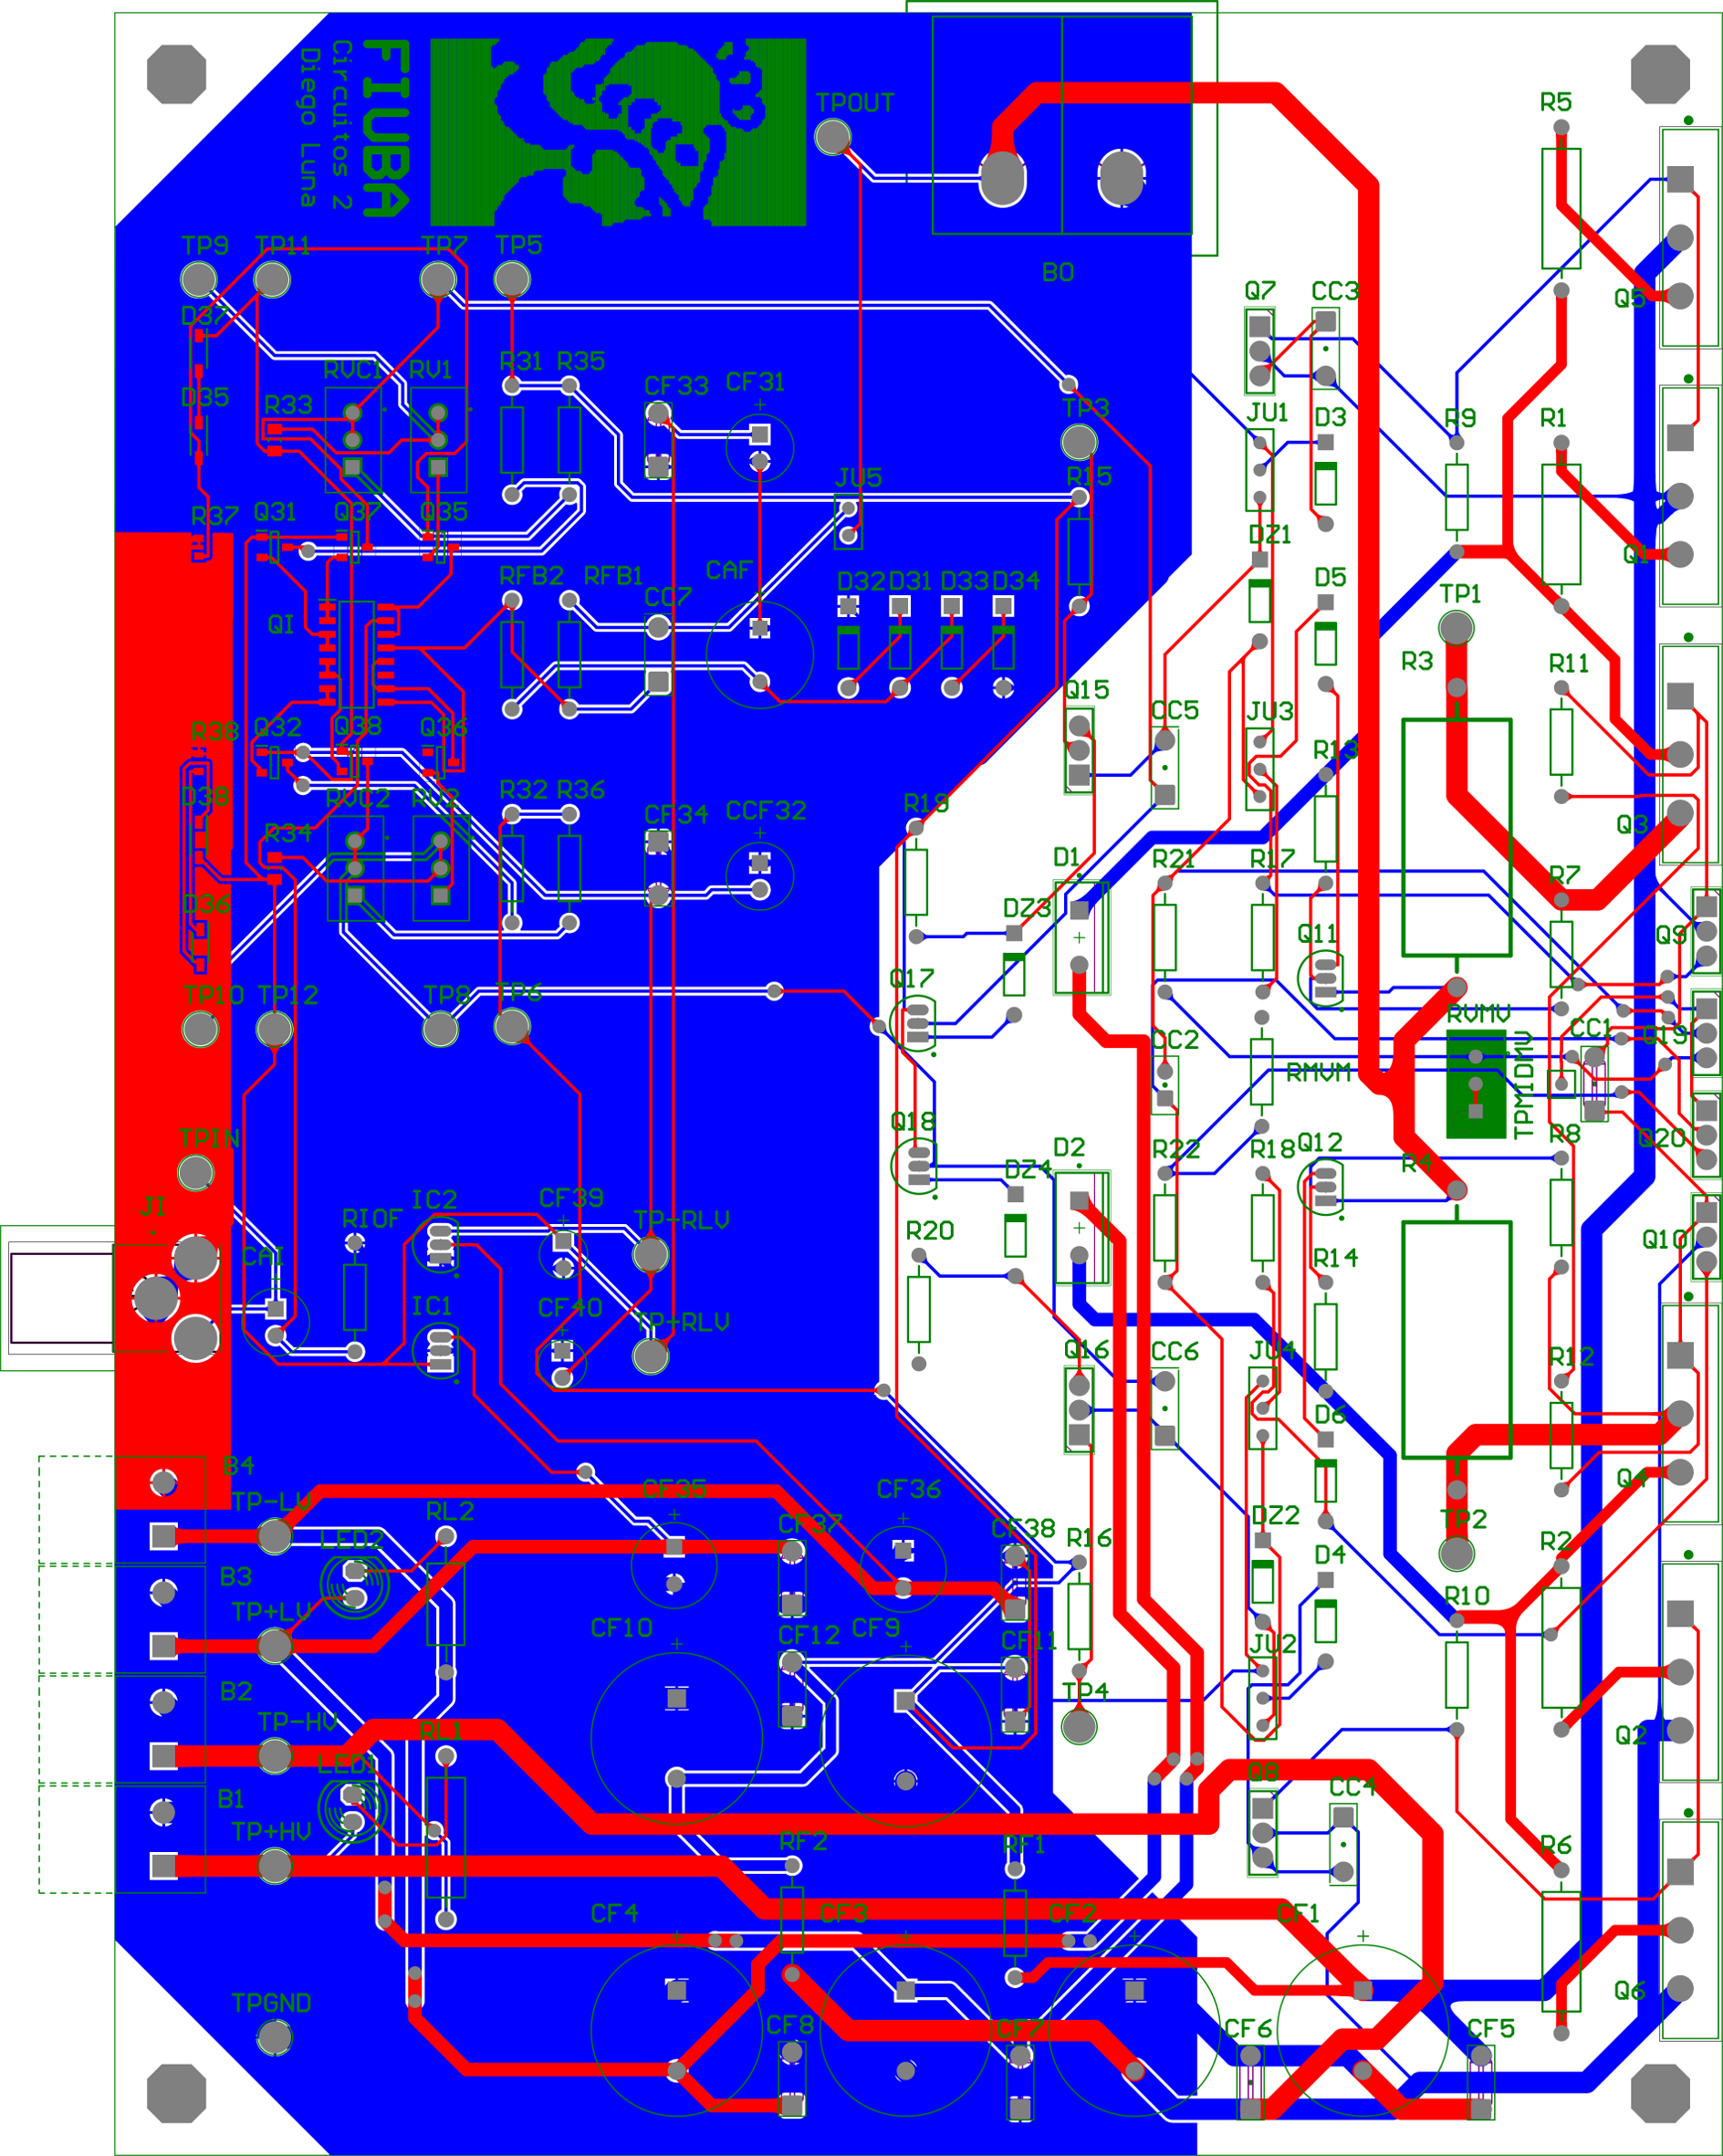
\includegraphics[height=200mm, angle=0]{img/PCB/layers/amplifier/all-2D.png}
    \caption{\footnotesize{Todas las capas}}
    \label{fig:pcb_amp_all}
\end{figure}

\clearpage

\begin{figure}[H]
    \centering
    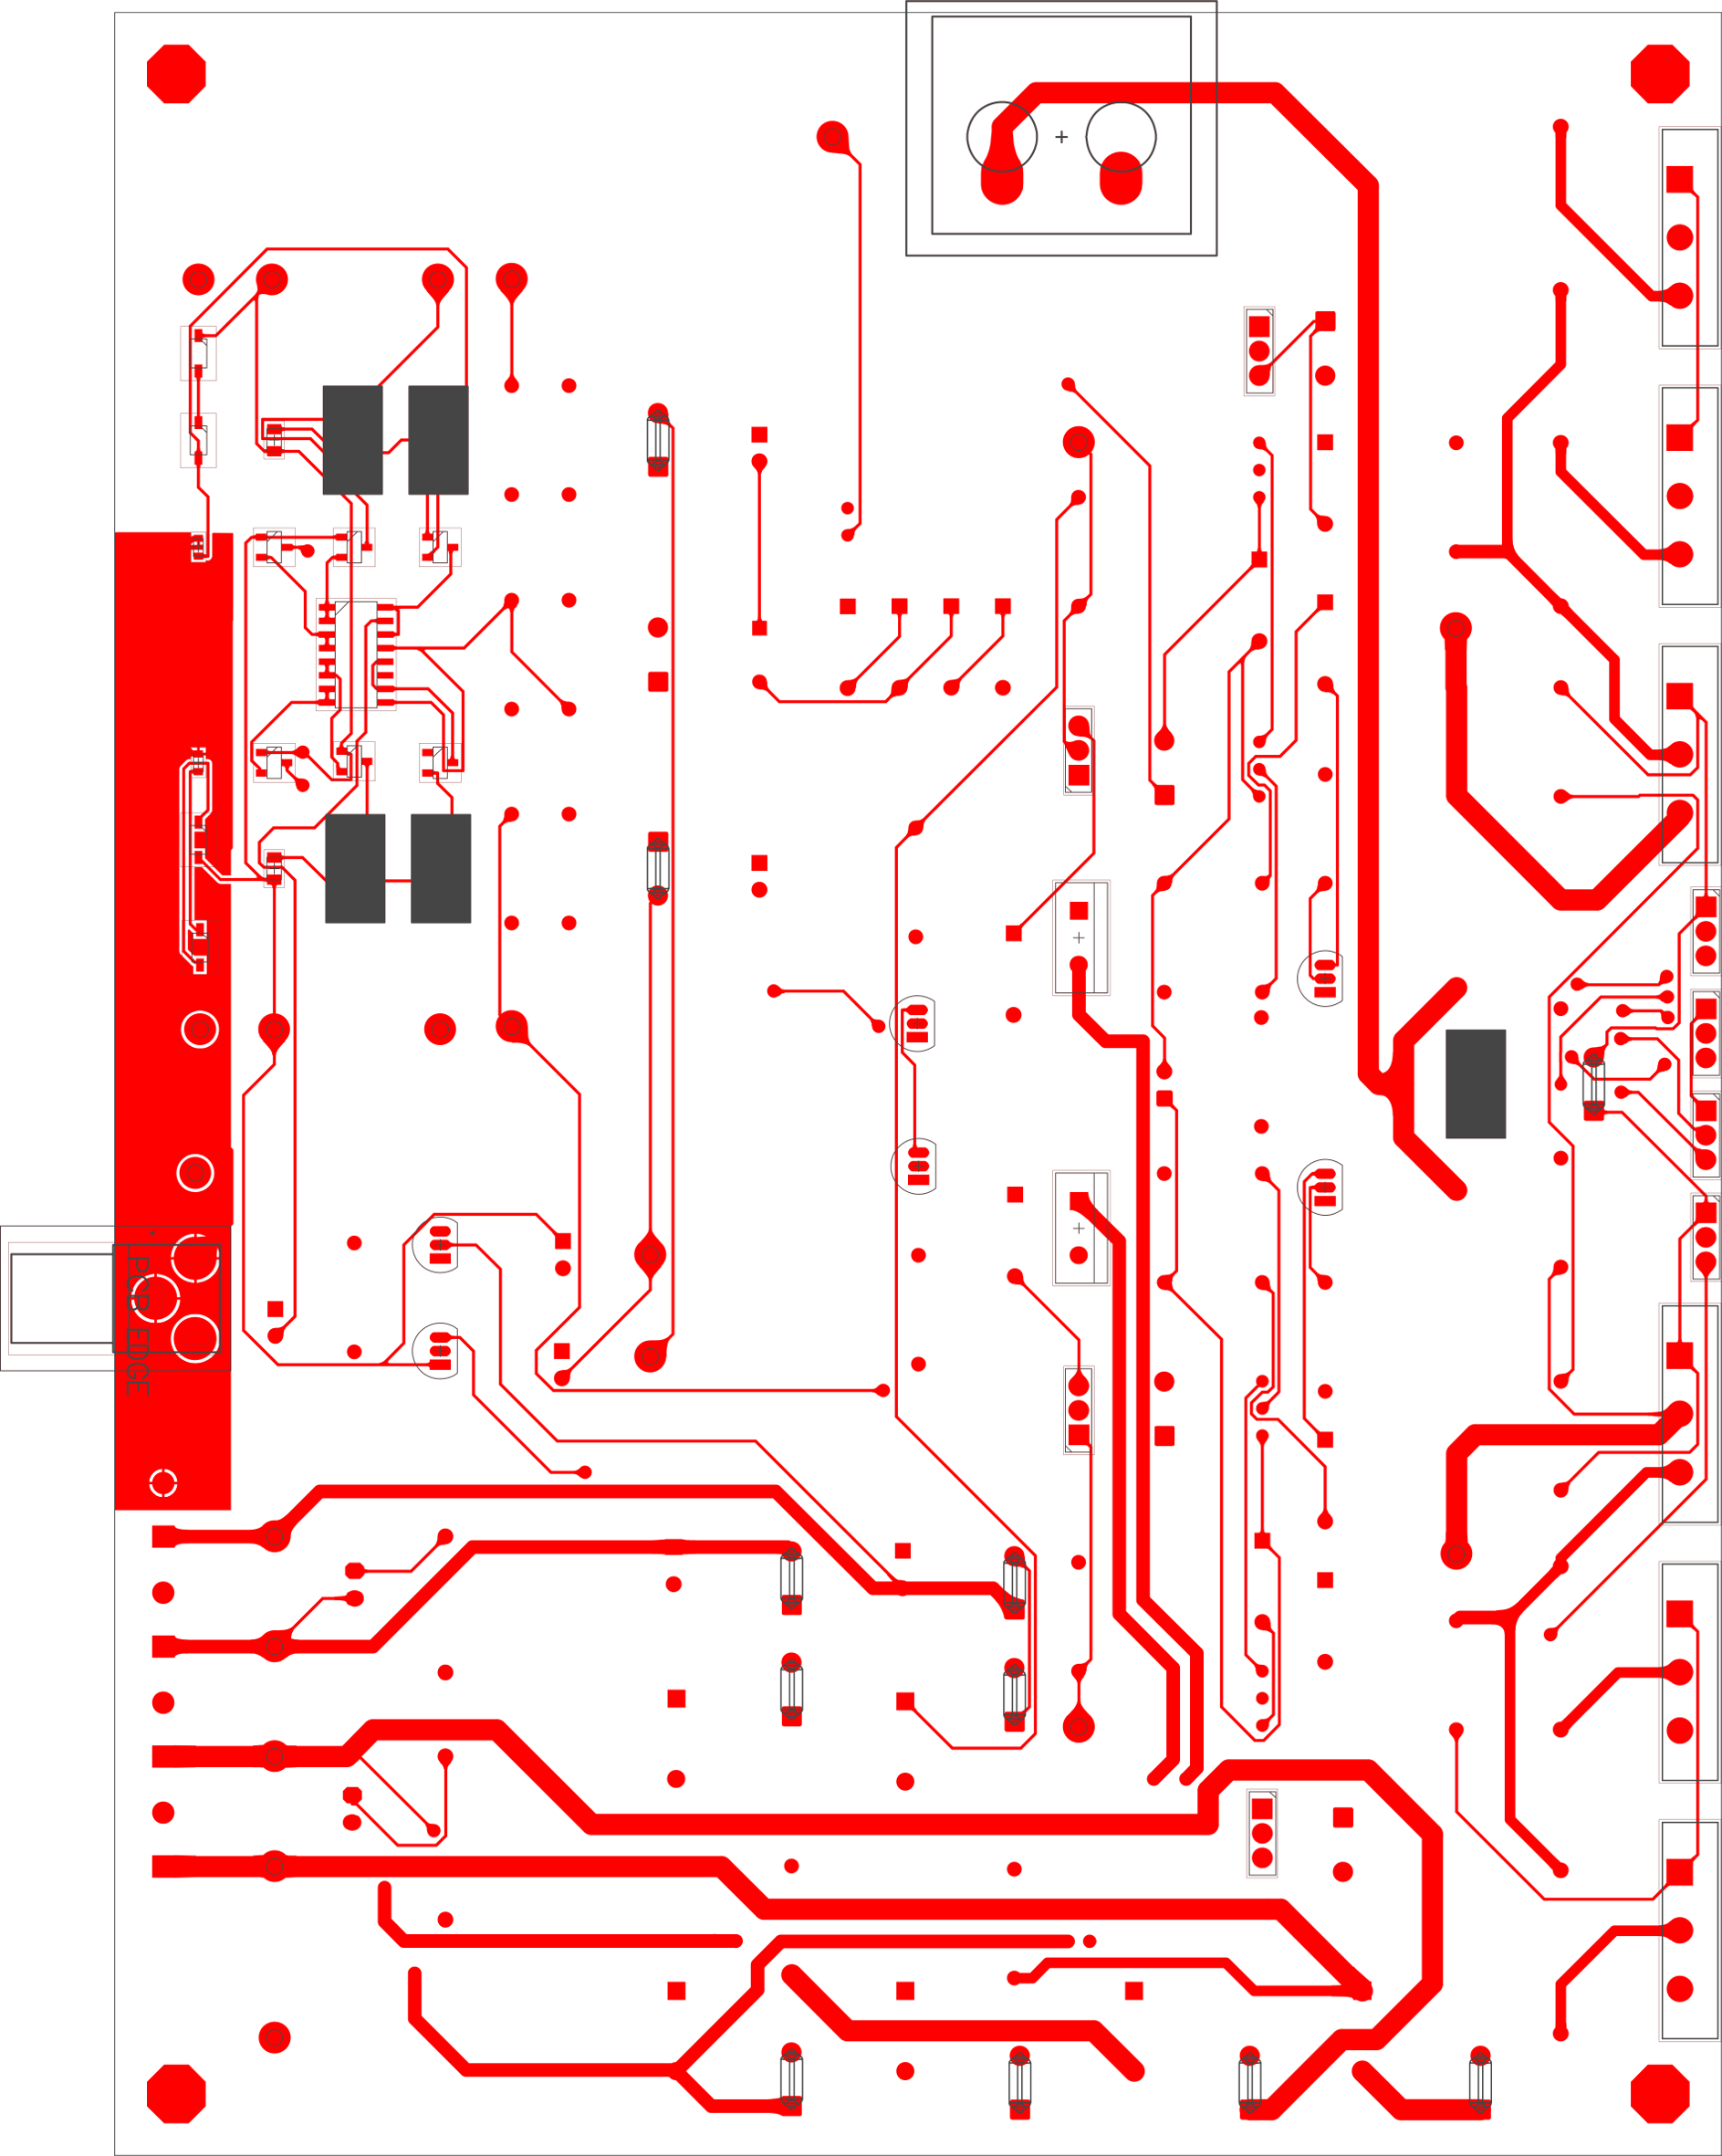
\includegraphics[height=200mm, angle=0]{img/PCB/layers/amplifier/top-copper.png}
    \caption{\footnotesize{Cobre superior}}
    \label{fig:pcb_amp_top_copper}
\end{figure}

\clearpage

\begin{figure}[H]
    \centering
    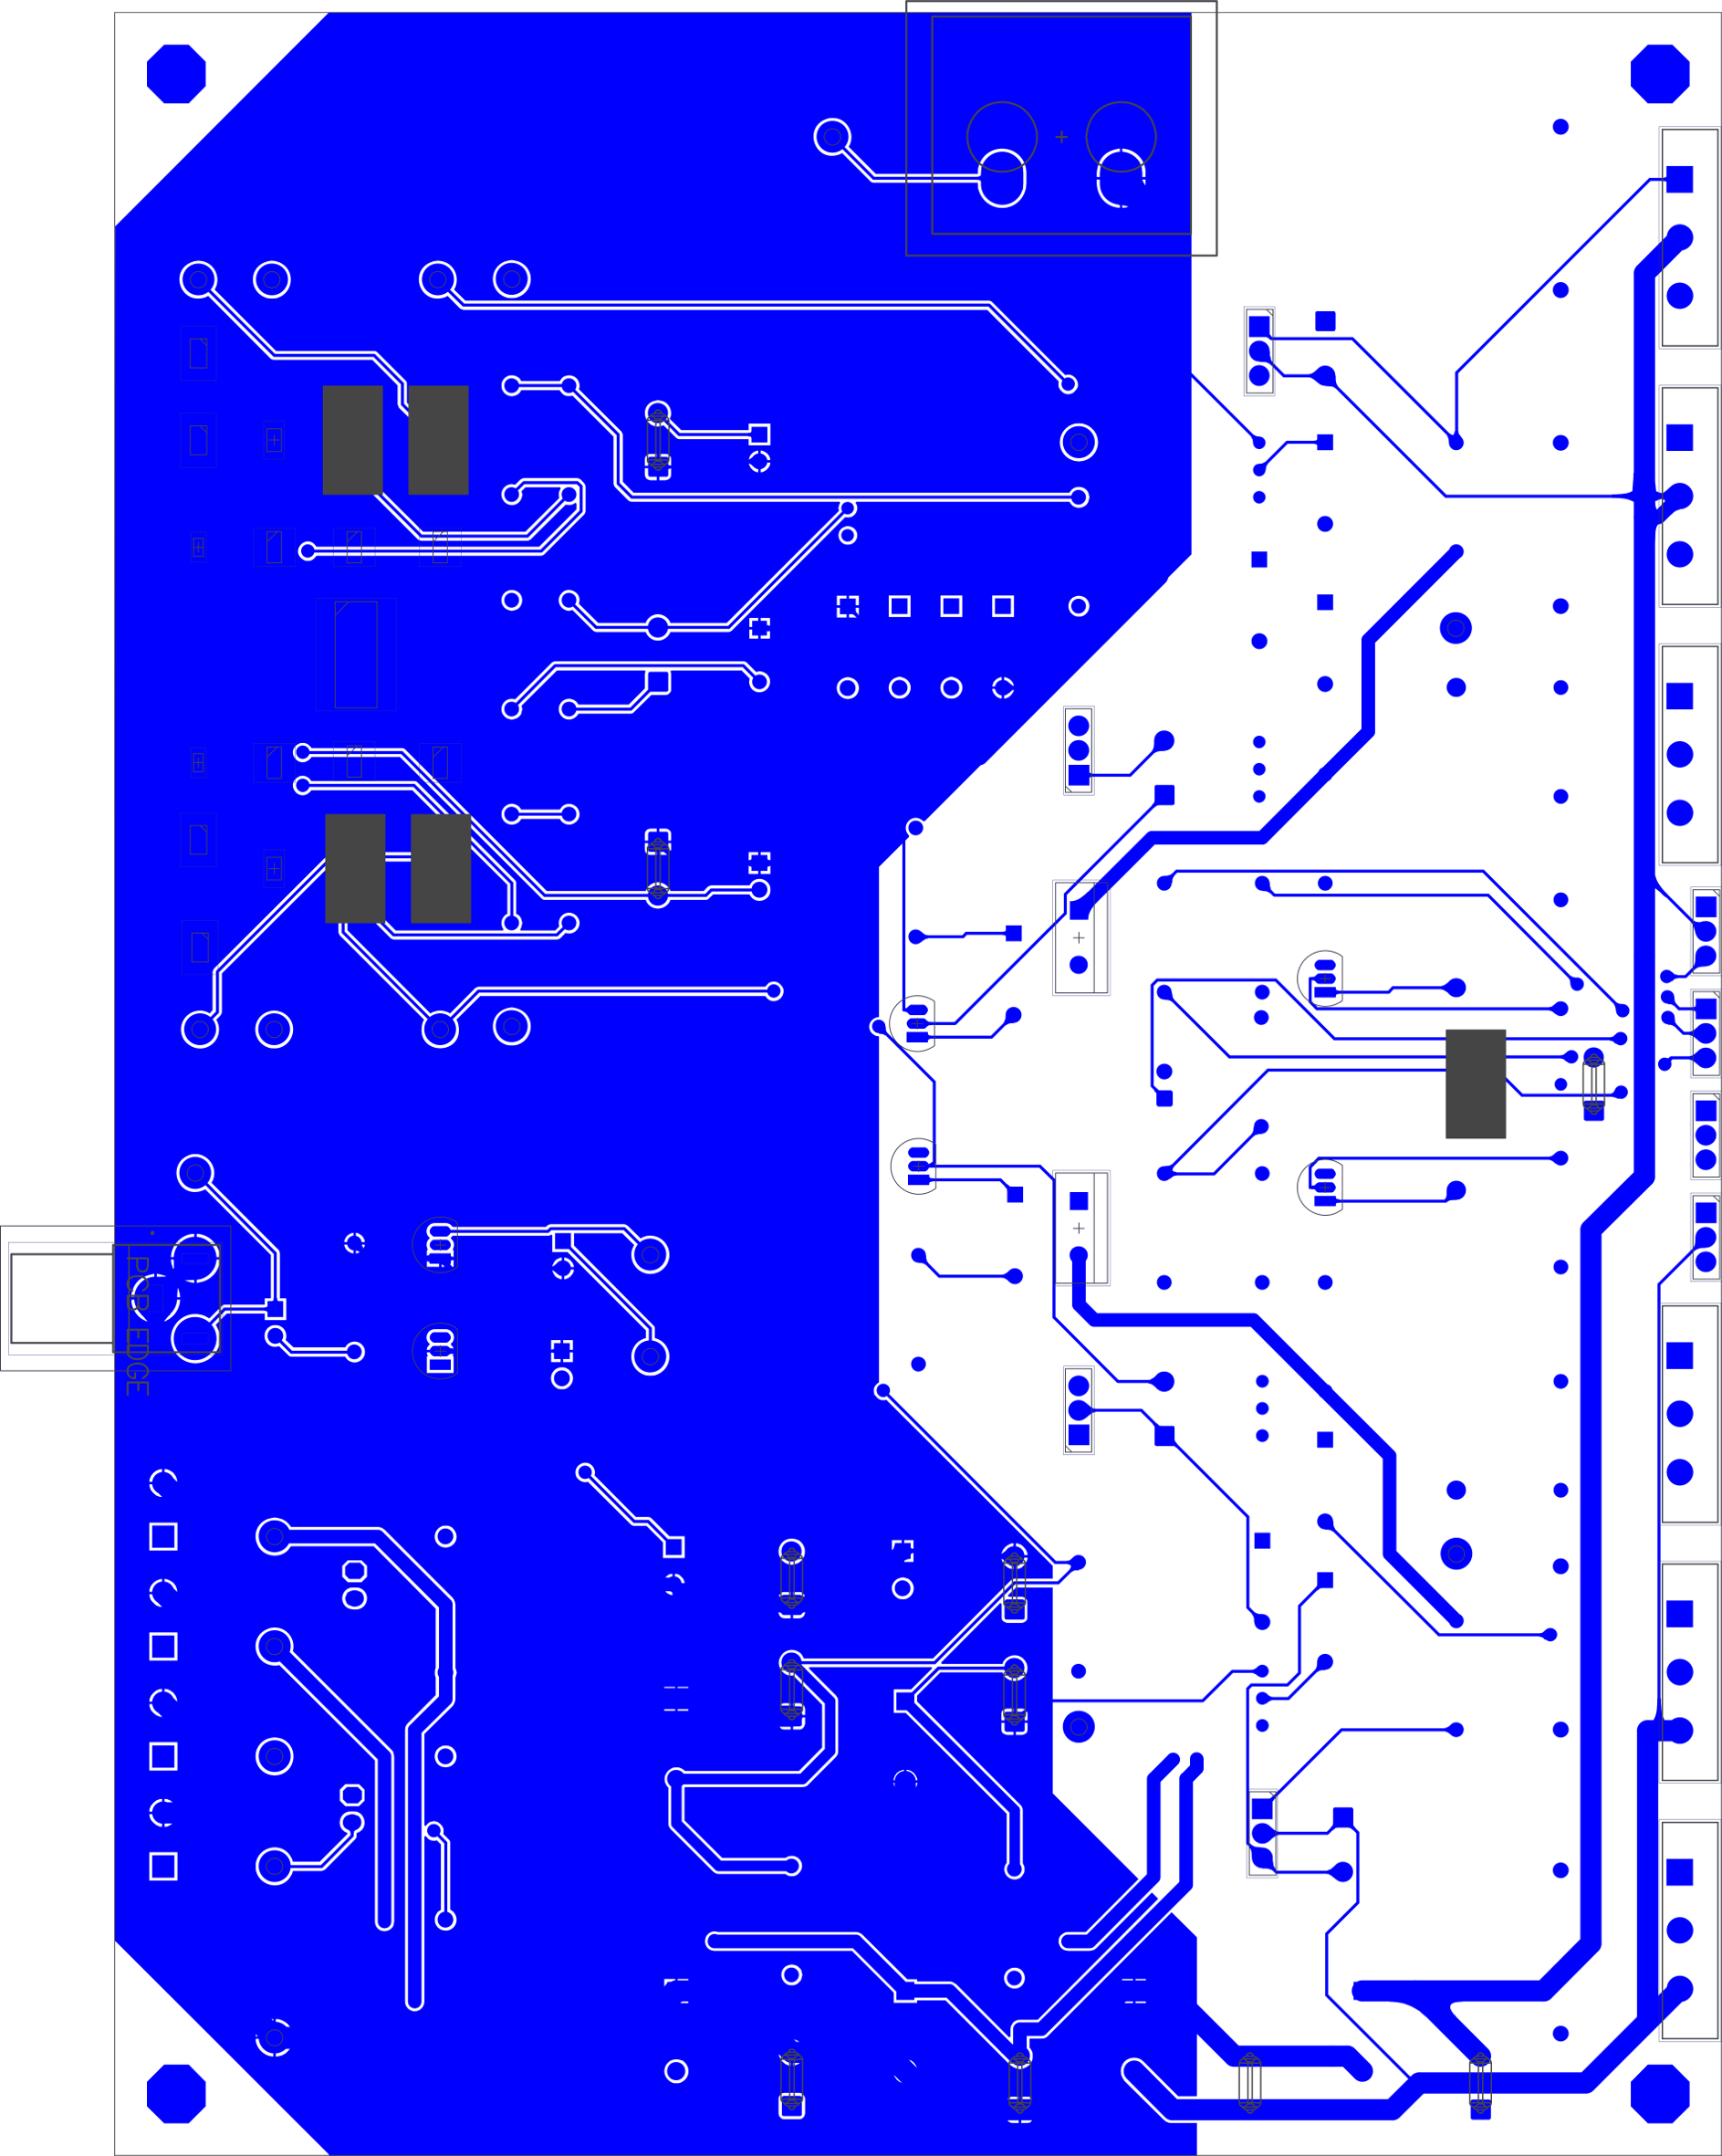
\includegraphics[height=200mm, angle=0]{img/PCB/layers/amplifier/bottom-copper.png}
    \caption{\footnotesize{Cobre inferior}}
    \label{fig:pcb_amp_bottom_copper}
\end{figure}

\clearpage

\begin{figure}[H]
    \centering
    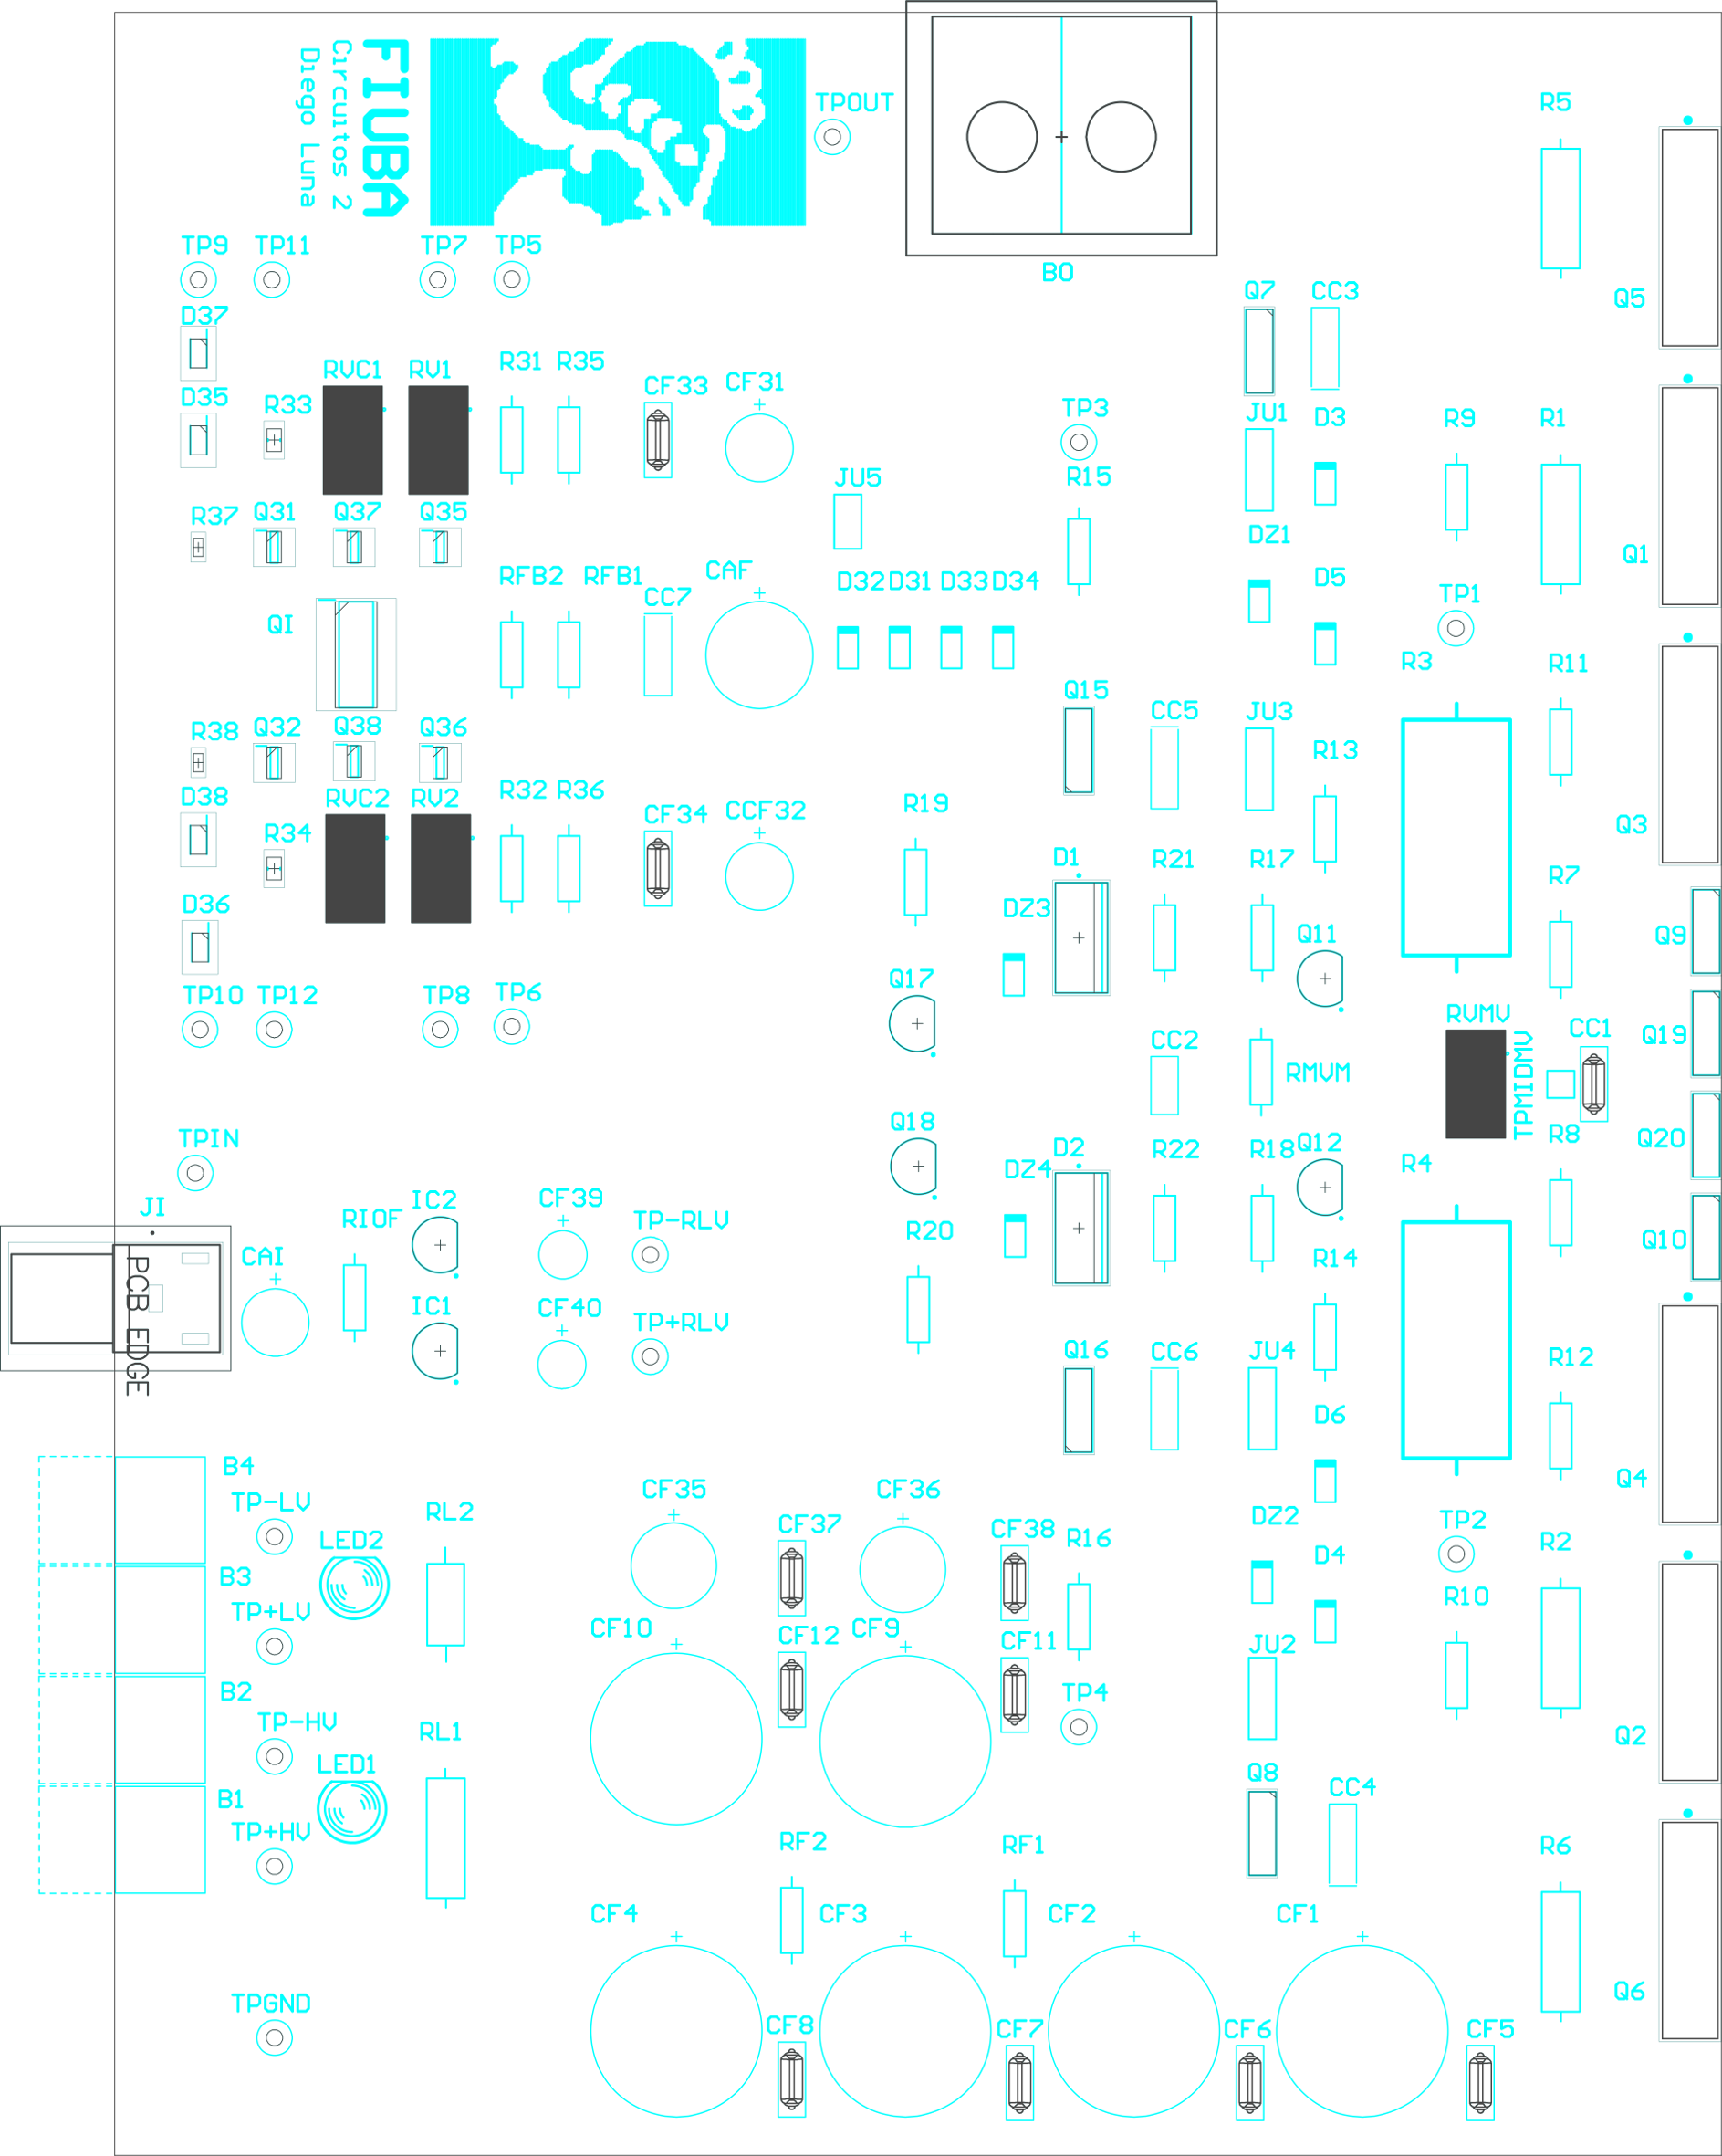
\includegraphics[height=200mm, angle=0]{img/PCB/layers/amplifier/top-overlay.png}
    \caption{\footnotesize{Componentes}}
    \label{fig:pcb_amp_top_overlay}
\end{figure}

\clearpage





\subsection{PCB del pre-amplificador}

En las siguientes páginas se incluyen las capas del PCB del pre-amplificador diseñado en Altium, ver archivo adjunto, \textbf{\quotemarks{PCBS-3D.pdf}} para una vista 3D interactiva del PCB.

\clearpage

\begin{figure}[H]
    \centering
    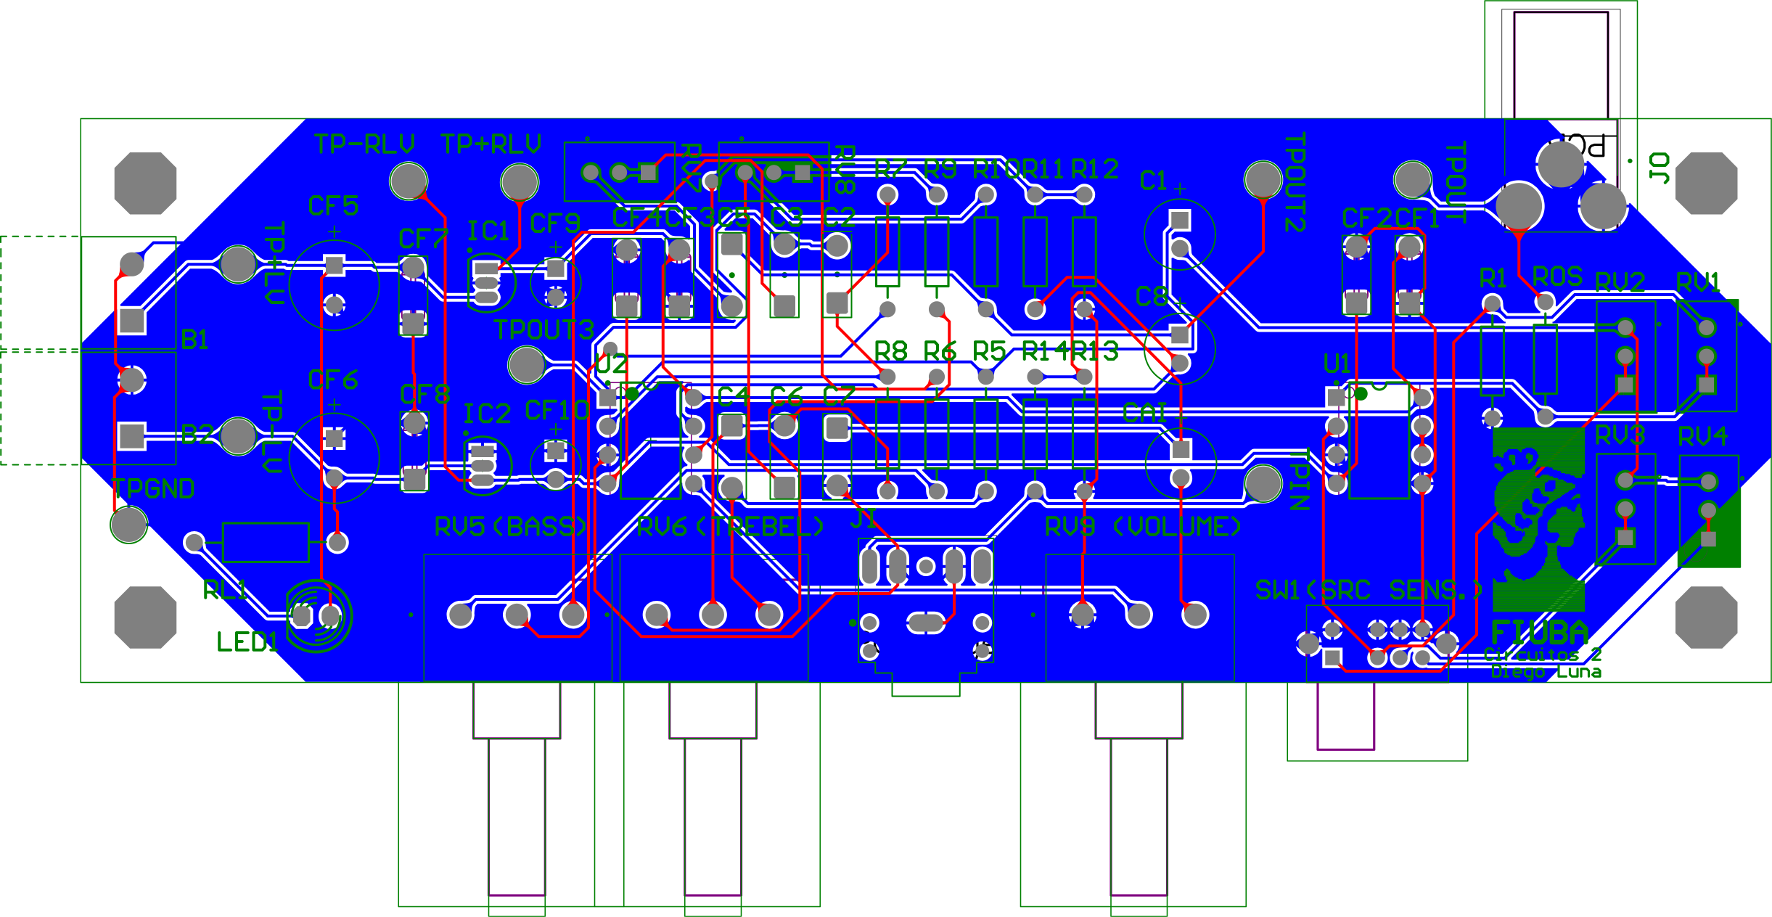
\includegraphics[width=150mm, angle=90]{img/PCB/layers/preamp/all-2D.png}
    \caption{\footnotesize{Todas las capas}}
    \label{fig:pcb_preamp_all}
\end{figure}

\clearpage

\begin{figure}[H]
    \centering
    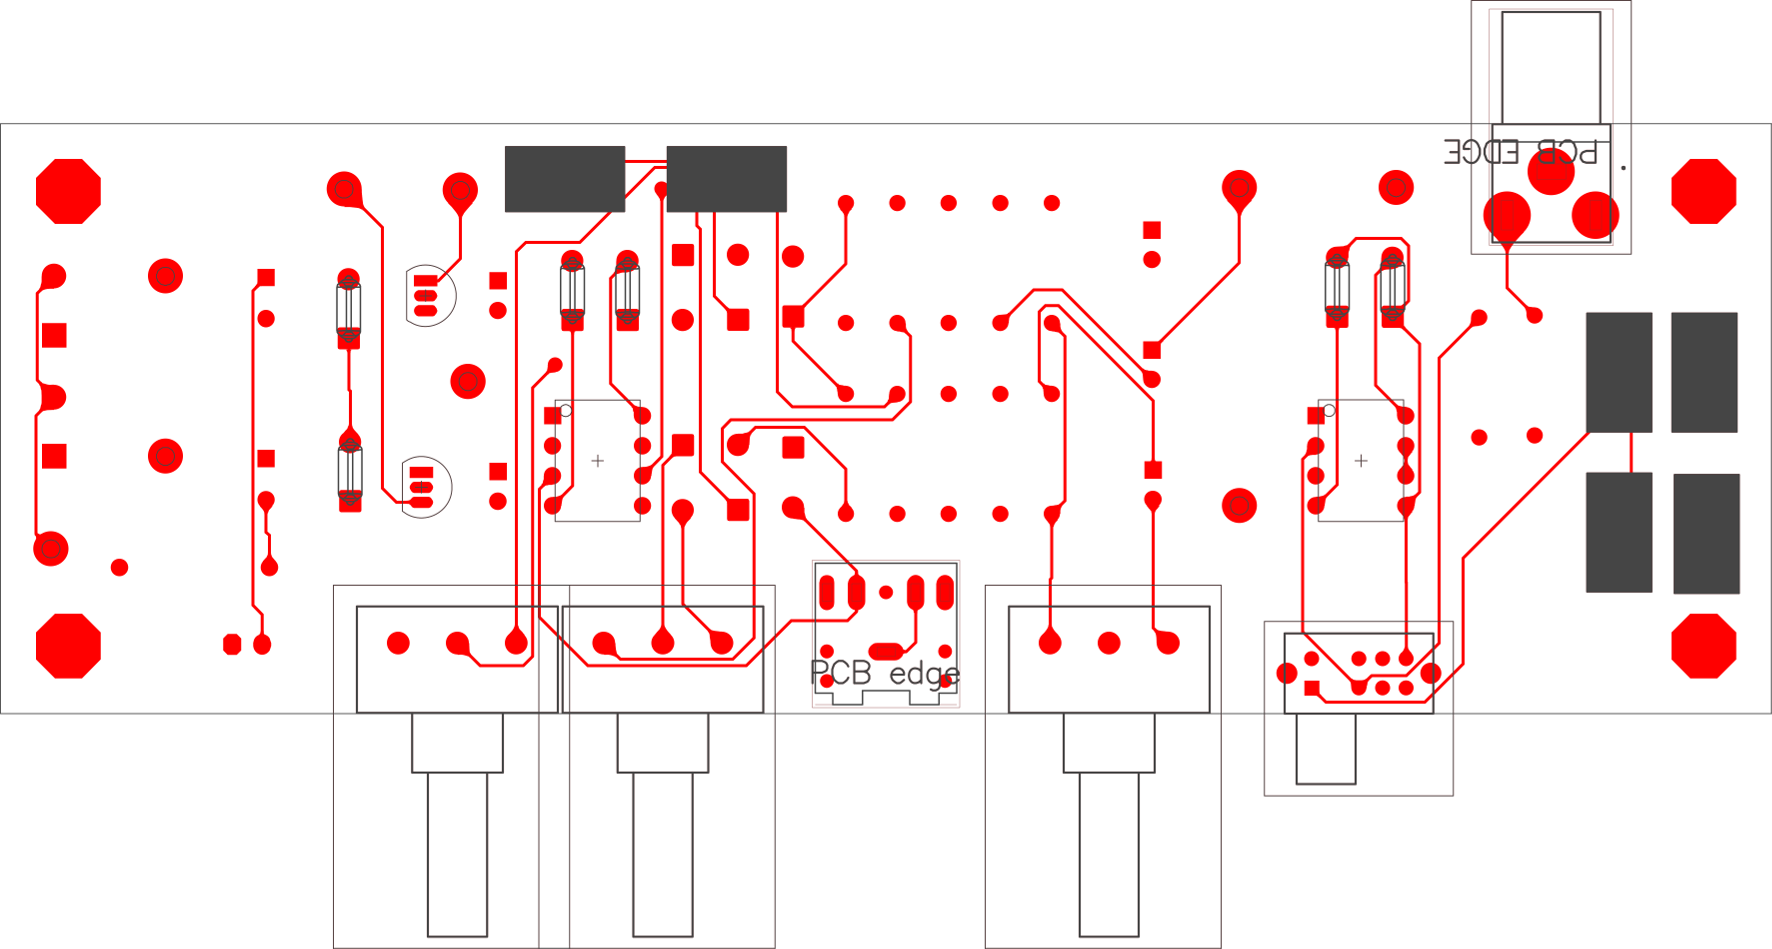
\includegraphics[width=150mm, angle=90]{img/PCB/layers/preamp/top-copper.png}
    \caption{\footnotesize{Cobre superior}}
    \label{fig:pcb_preamp_top_copper}
\end{figure}

\clearpage

\begin{figure}[H]
    \centering
    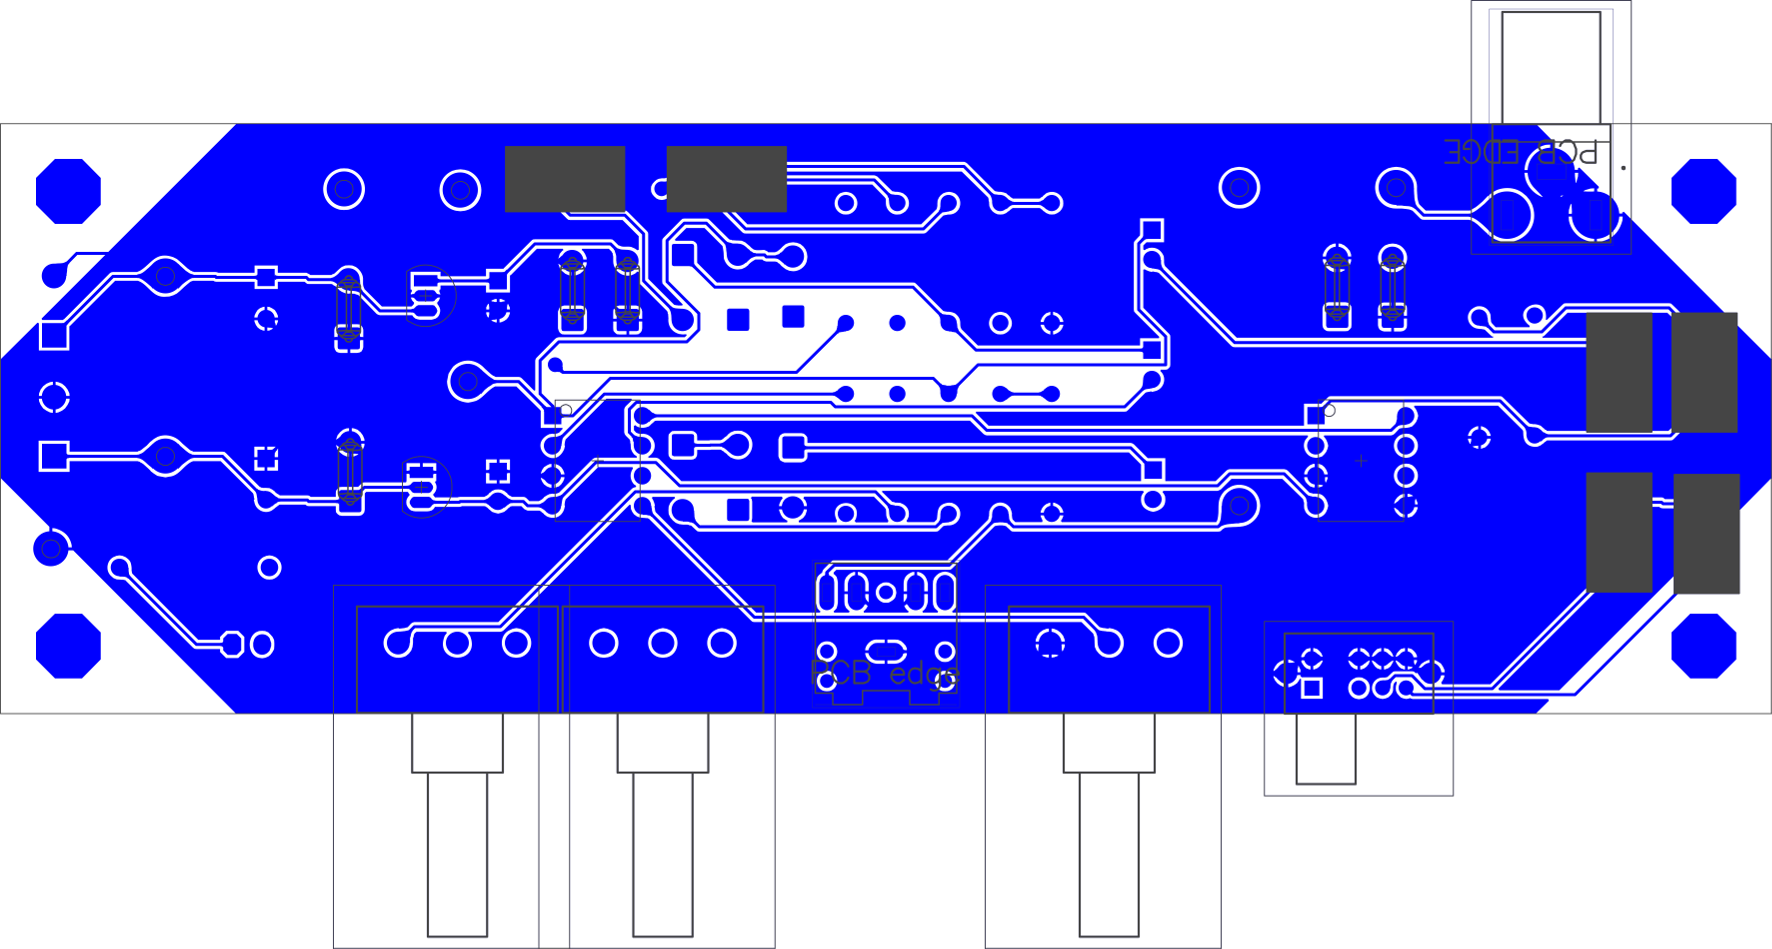
\includegraphics[width=150mm, angle=90]{img/PCB/layers/preamp/bottom-copper.png}
    \caption{\footnotesize{Cobre inferior}}
    \label{fig:pcb_preamp_bottom_copper}
\end{figure}

\clearpage

\begin{figure}[H]
    \centering
    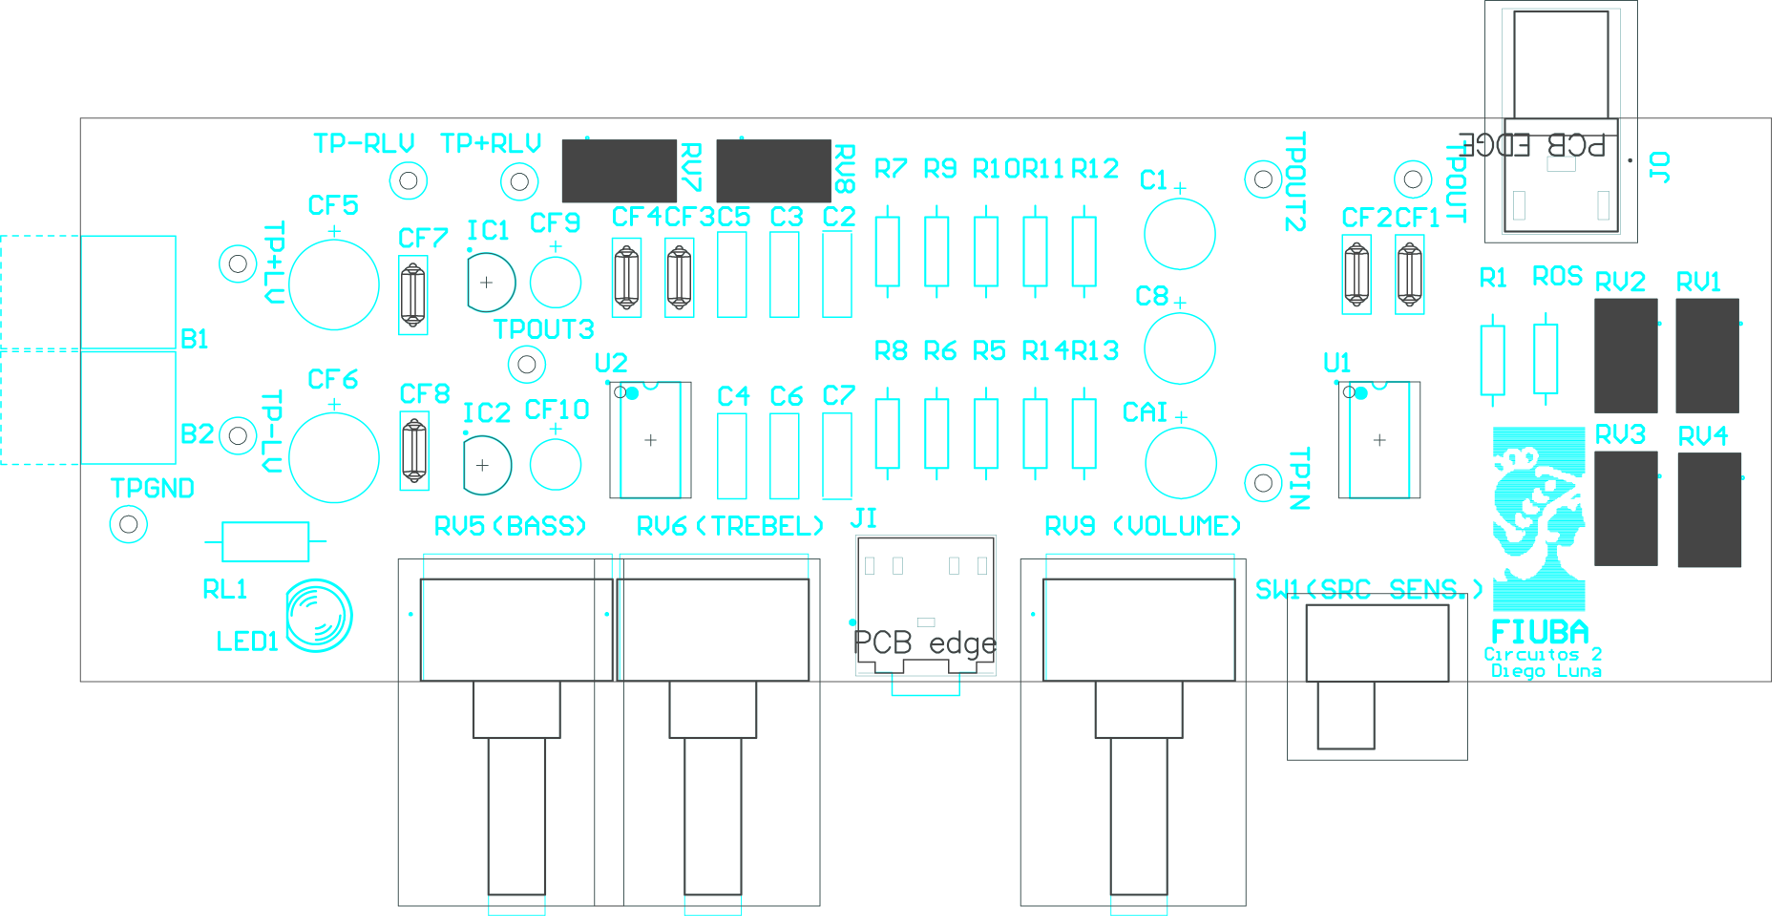
\includegraphics[width=150mm, angle=90]{img/PCB/layers/preamp/top-overlay.png}
    \caption{\footnotesize{Componentes}}
    \label{fig:pcb_preamp_top_overlay}
\end{figure}

\clearpage



\subsection{PCB de la fuente de alimentación}

En las siguientes páginas se incluyen las capas del PCB de la fuente de alimentación diseñada en Altium, ver archivo adjunto, \textbf{\quotemarks{PCBS-3D.pdf}} para una vista 3D interactiva del PCB.

\clearpage

\begin{figure}[H]
    \centering
    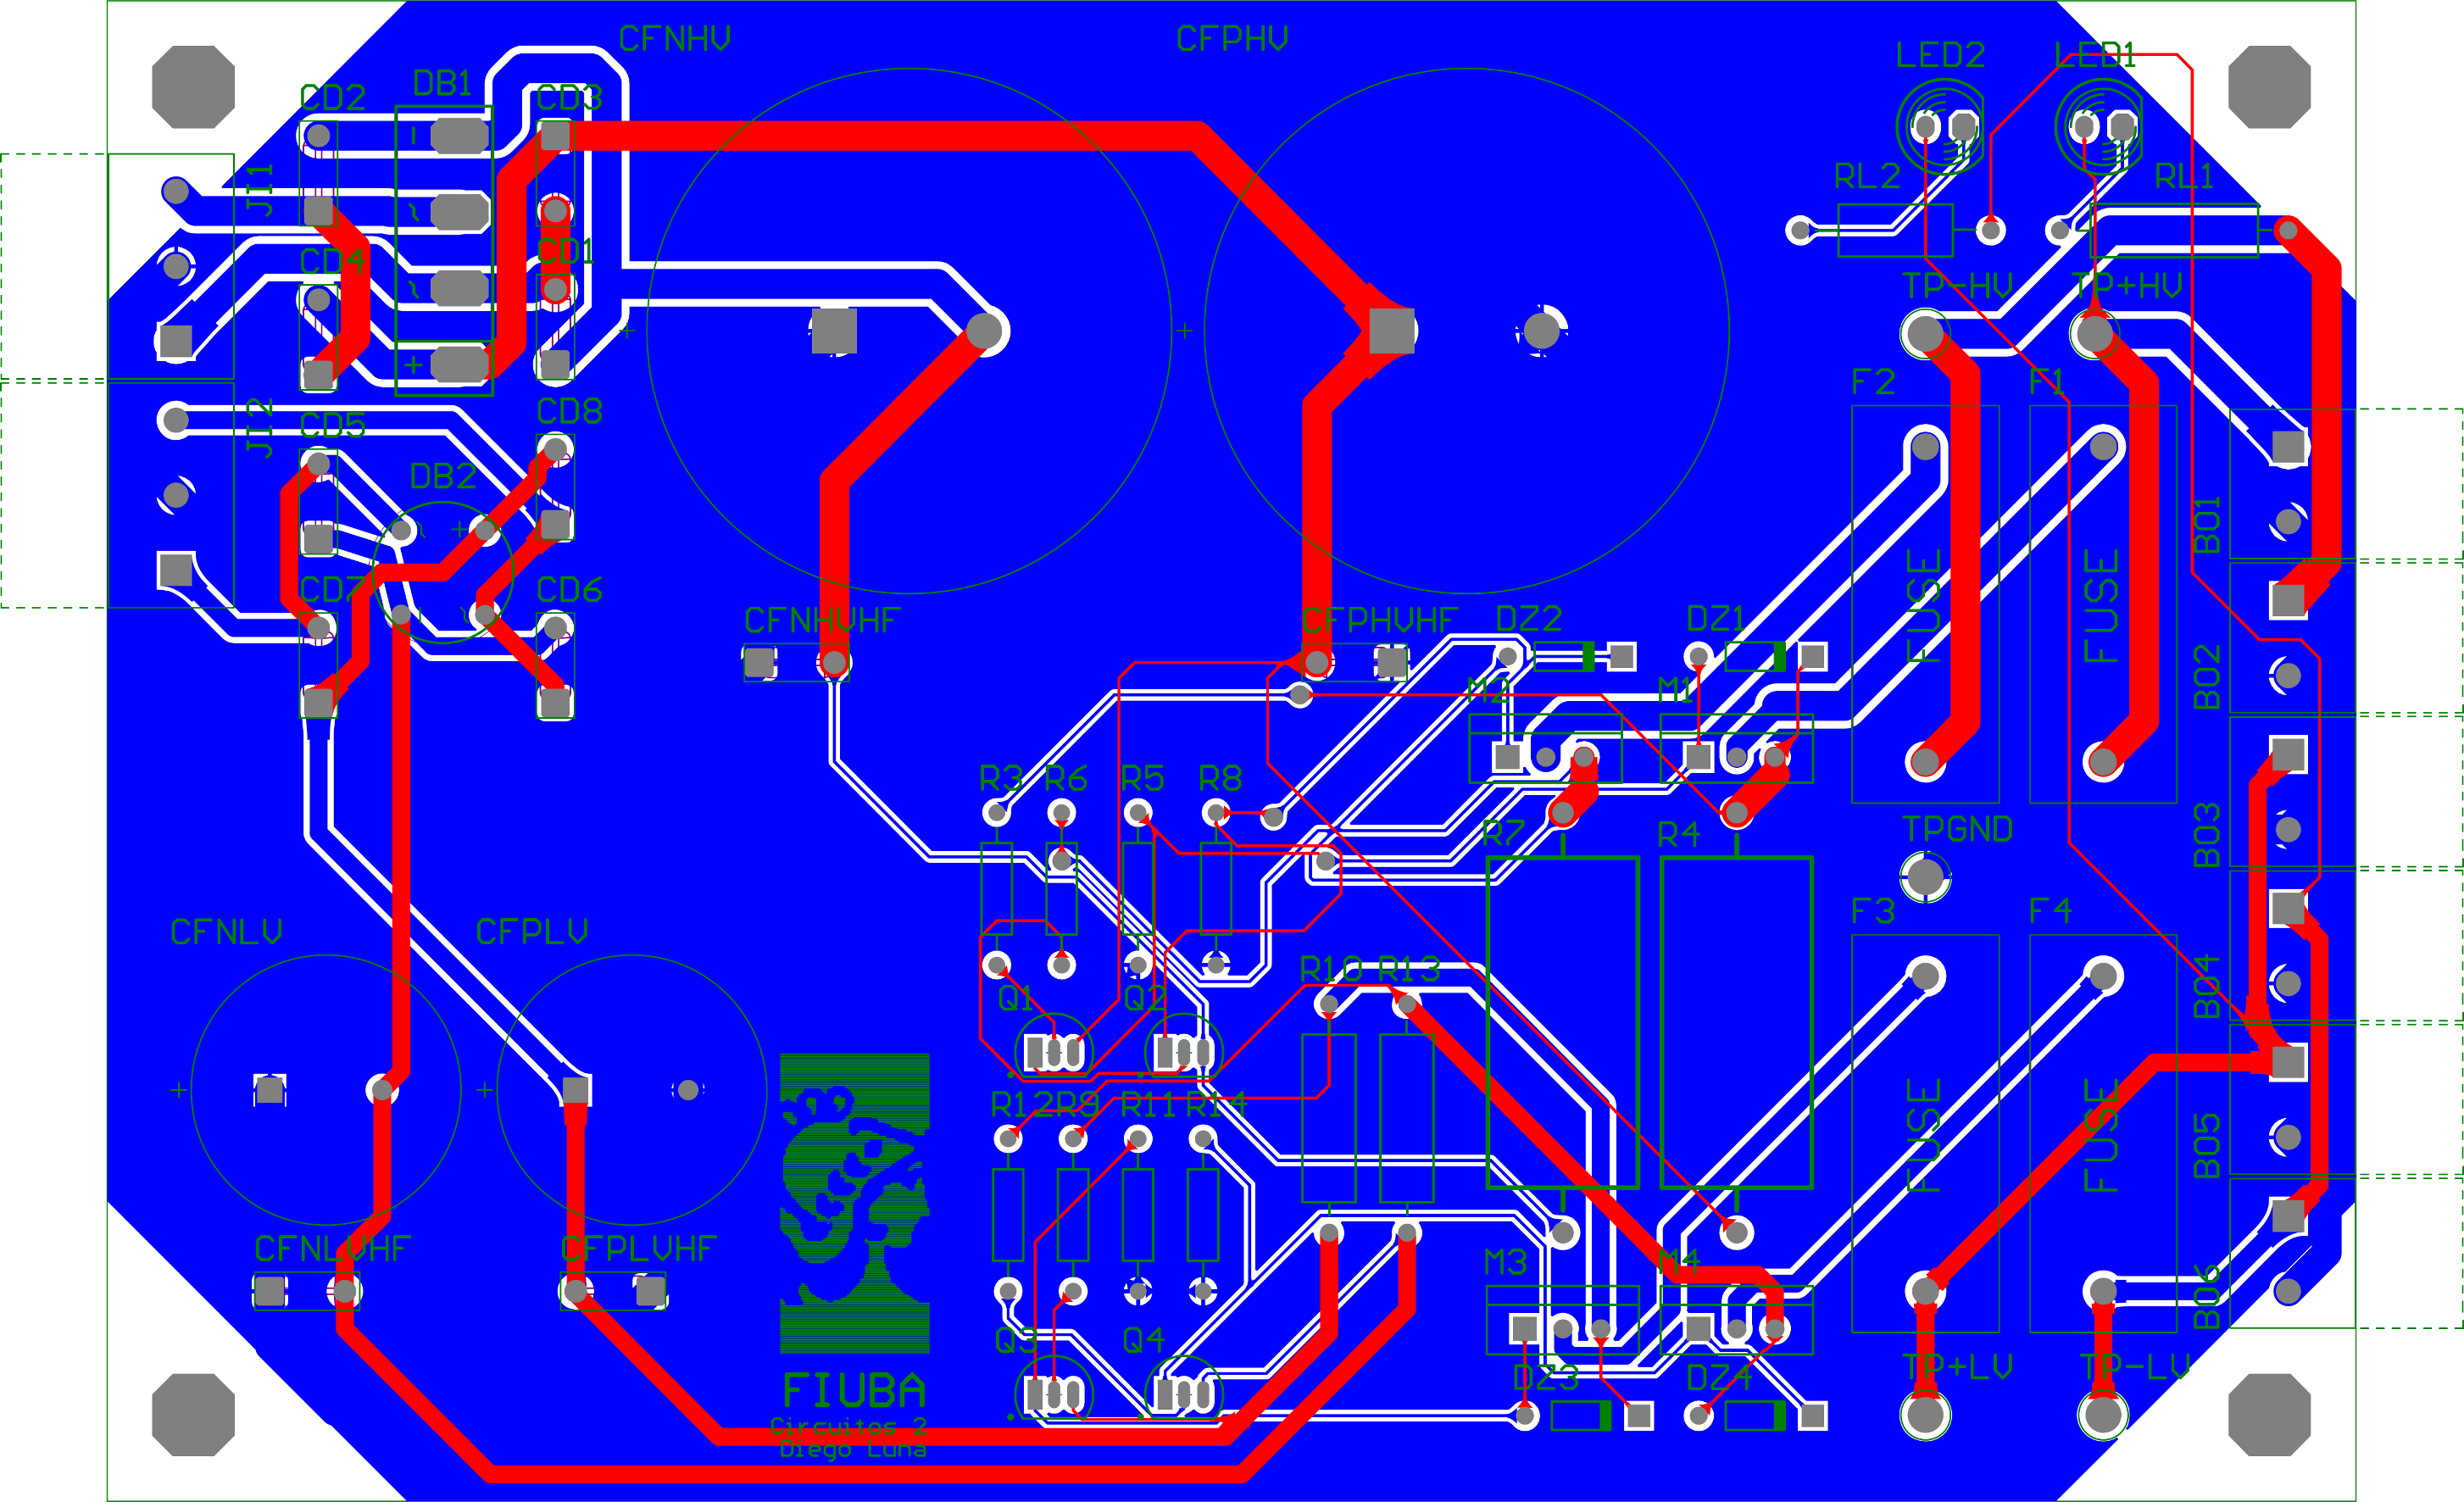
\includegraphics[width=150mm, angle=90]{img/PCB/layers/power_supply/all-2D.png}
    \caption{\footnotesize{Todas las capas}}
    \label{fig:pcb_preamp_all}
\end{figure}

\clearpage

\begin{figure}[H]
    \centering
    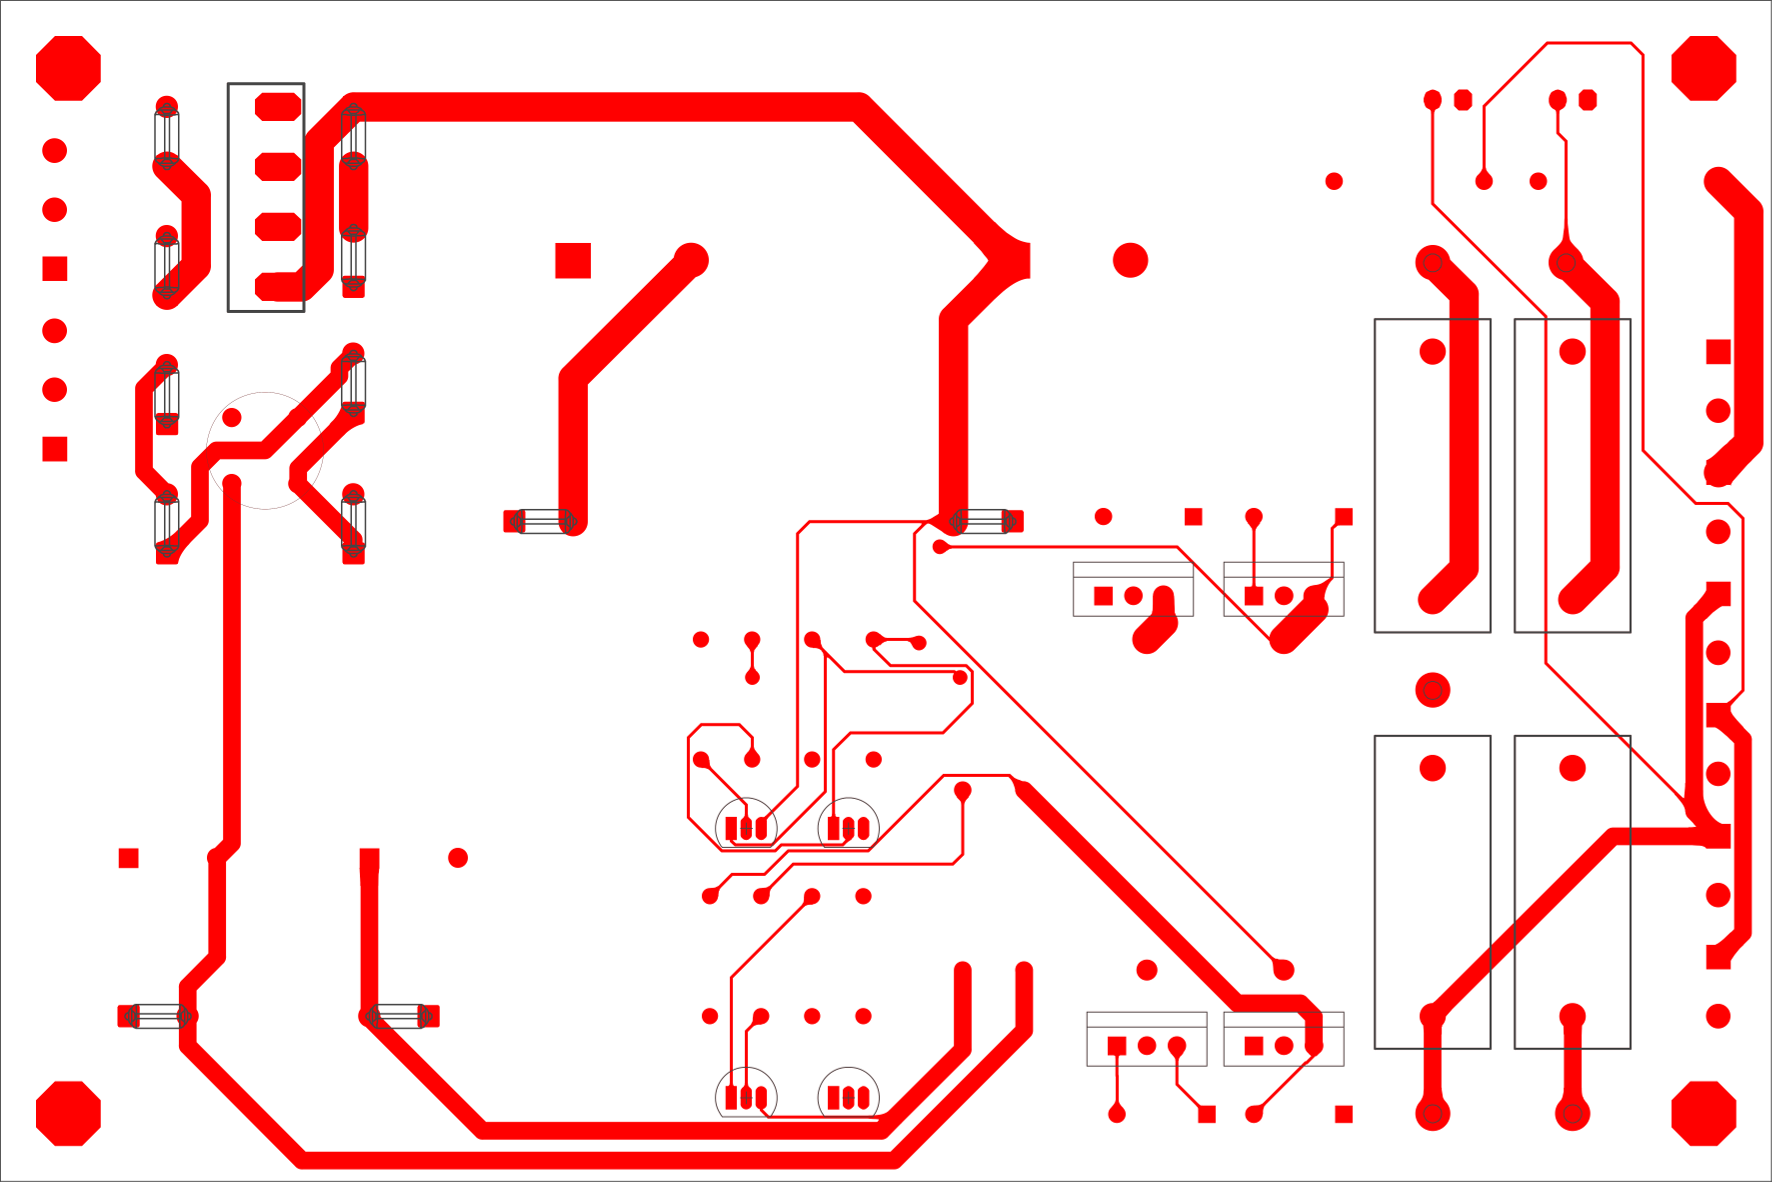
\includegraphics[width=150mm, angle=90]{img/PCB/layers/power_supply/top-copper.png}
    \caption{\footnotesize{Cobre superior}}
    \label{fig:pcb_preamp_top_copper}
\end{figure}

\clearpage

\begin{figure}[H]
    \centering
    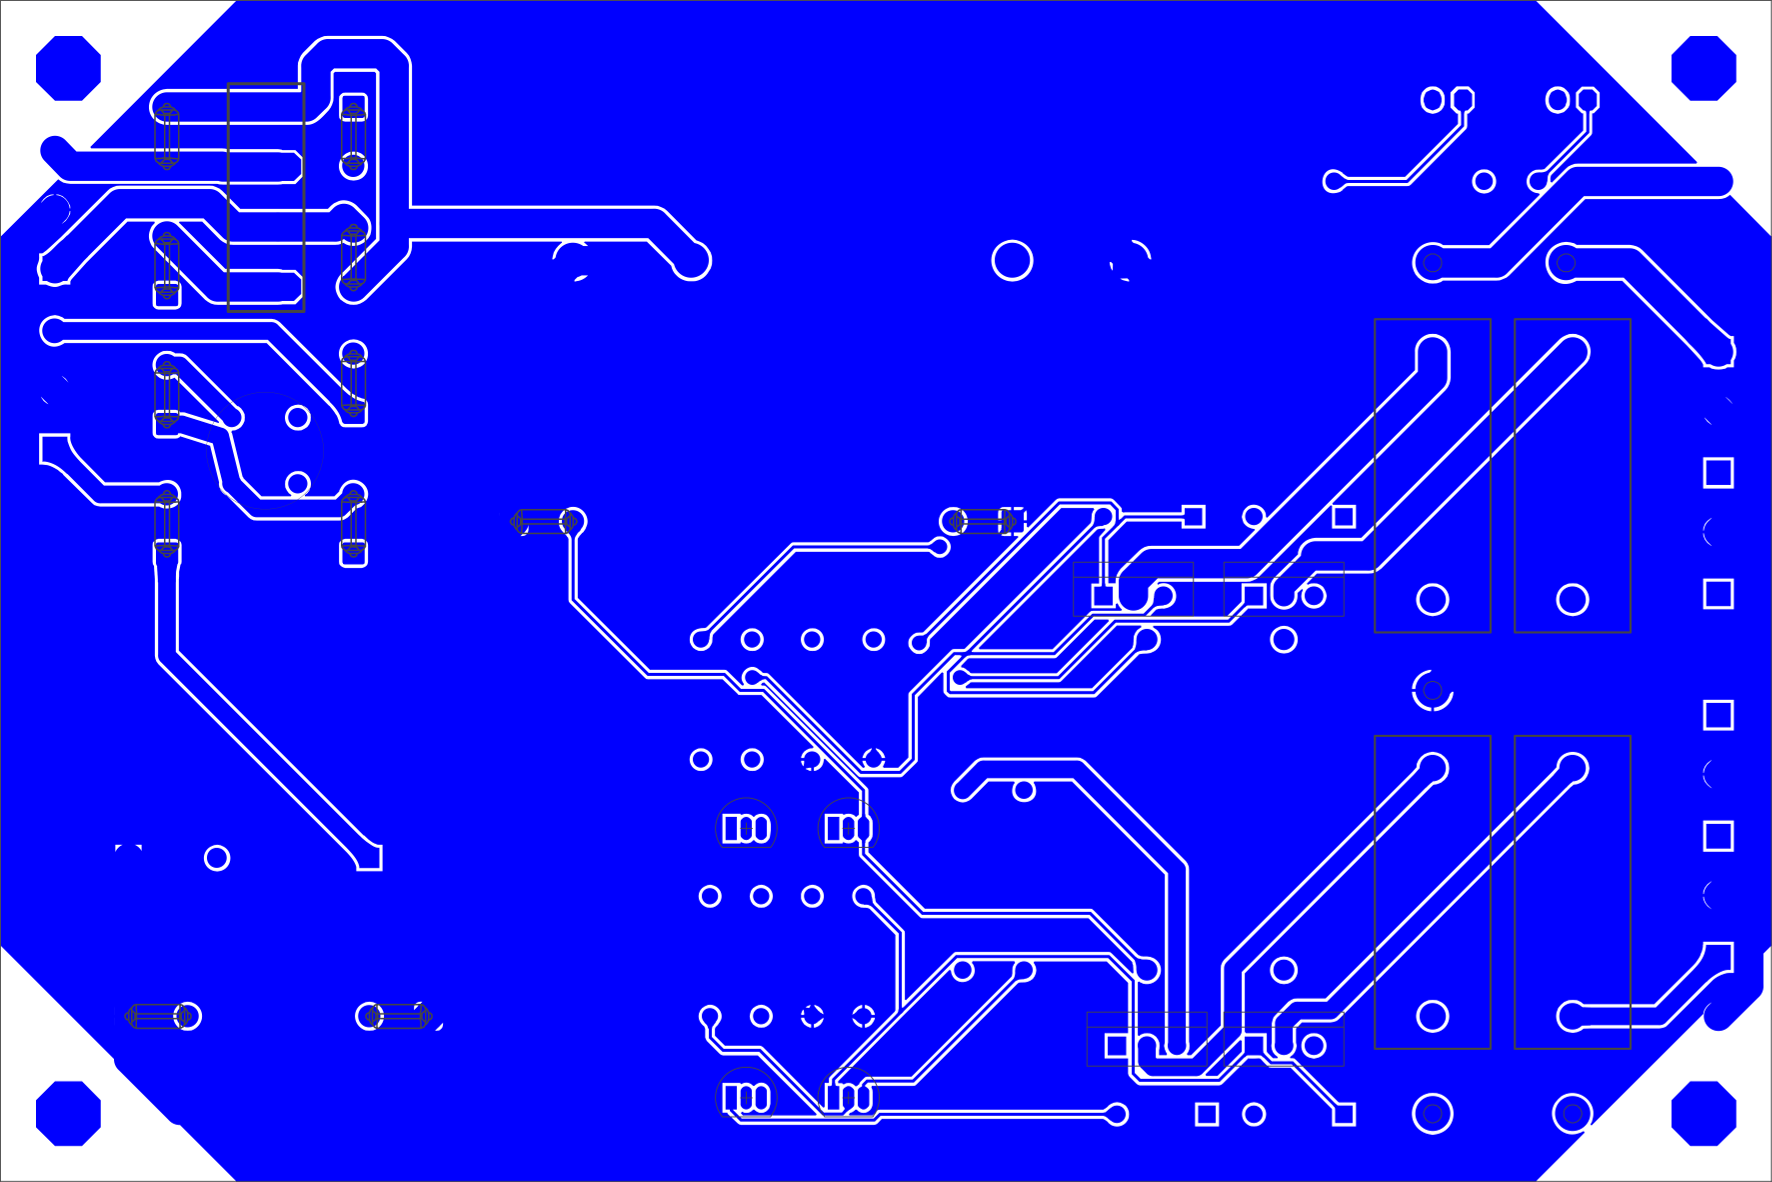
\includegraphics[width=150mm, angle=90]{img/PCB/layers/power_supply/bottom-copper.png}
    \caption{\footnotesize{Cobre inferior}}
    \label{fig:pcb_preamp_bottom_copper}
\end{figure}

\clearpage

\begin{figure}[H]
    \centering
    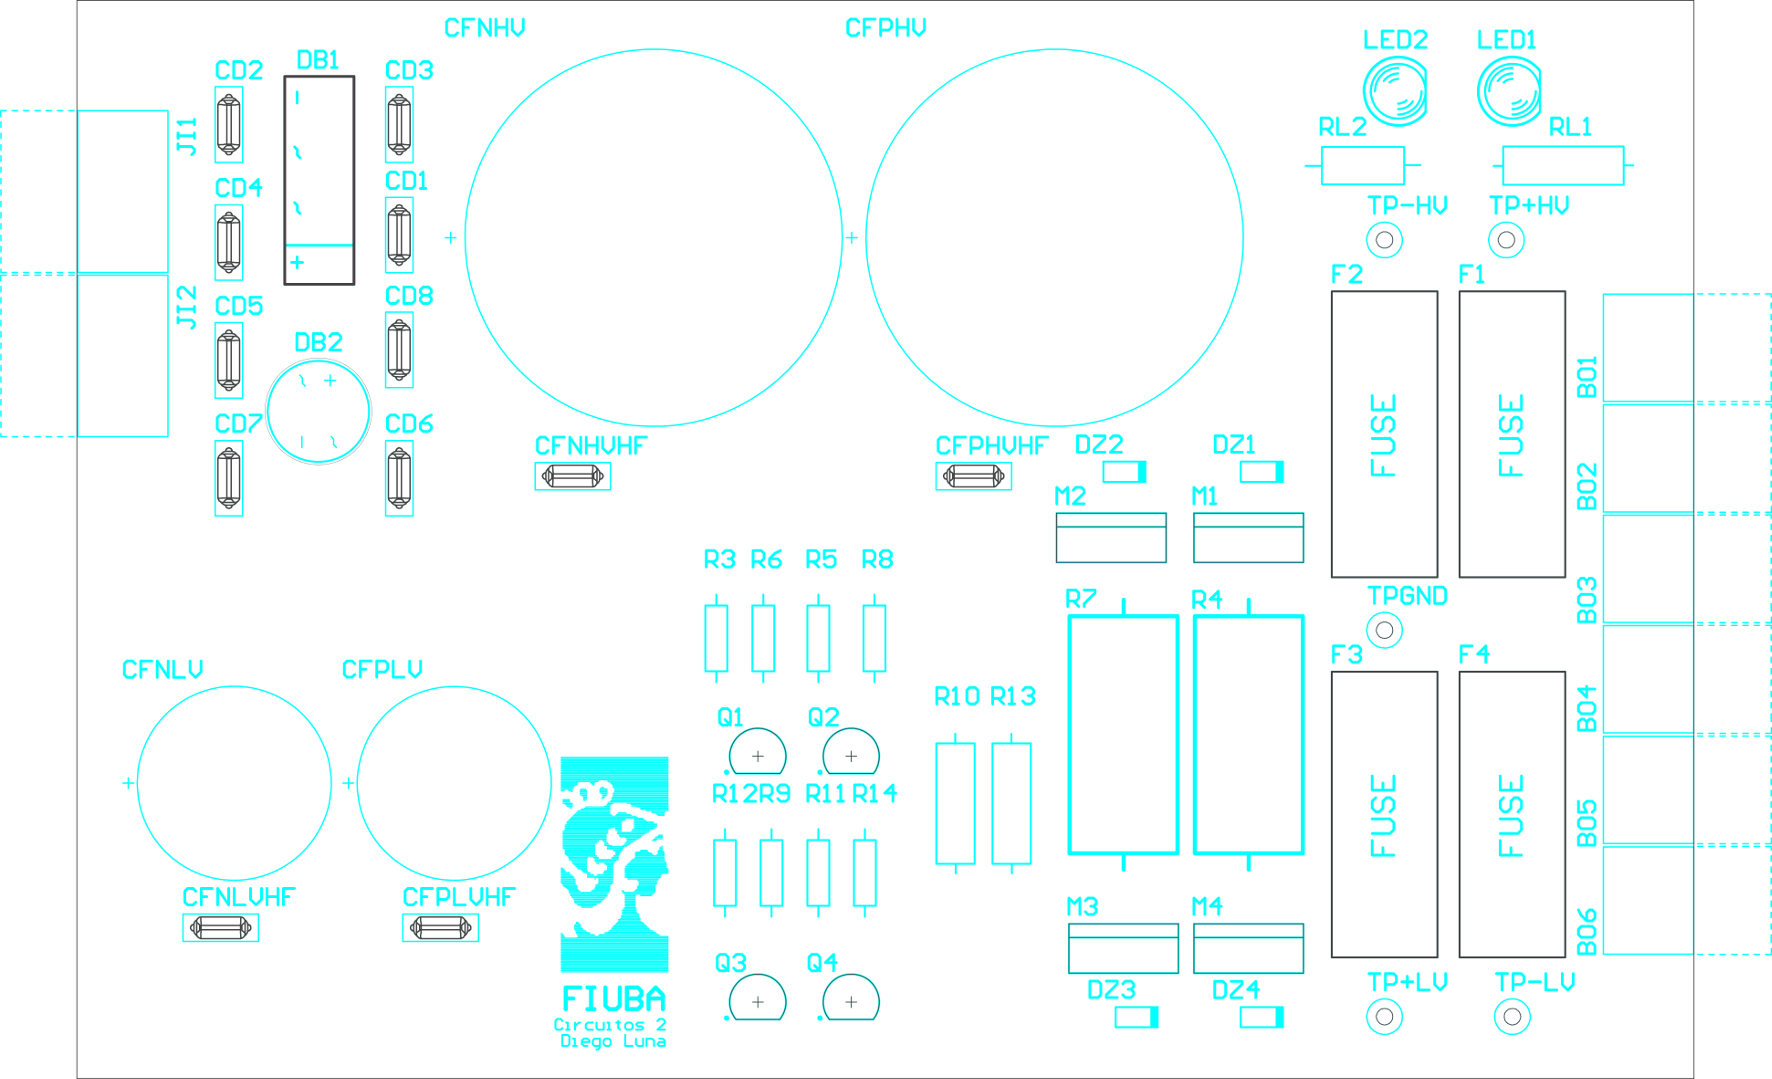
\includegraphics[width=150mm, angle=90]{img/PCB/layers/power_supply/top-overlay.png}
    \caption{\footnotesize{Componentes}}
    \label{fig:pcb_preamp_top_overlay}
\end{figure}

\clearpage
















